\documentclass[11pt, a4paper]{article}

% --- Packages ---
\usepackage[utf8]{inputenc}
\usepackage[T1]{fontenc}
\usepackage[english]{babel}
\usepackage{geometry}
\geometry{margin=2.5cm}
\usepackage{amsmath, amssymb, amsfonts}
\usepackage{graphicx}
\usepackage{booktabs}
\usepackage{hyperref}
\usepackage{cite}
\usepackage{titlesec}
\usepackage[section]{placeins}

% --- Hyperref Setup ---
\hypersetup{
    colorlinks=true,
    linkcolor=blue,
    filecolor=magenta,      
    urlcolor=cyan,
    citecolor=blue,
}

\begin{document}

% ==========================================
% TITLE PAGE
% ==========================================
\begin{titlepage}
    \centering
    \vspace*{2cm}

    {\Large \textsc{Ensemble Learning -- Research Project (2026/2027)}}\\[0.5cm]
    {\large Instructor: Stanisław Kaźmierczak}\\[3cm]

    % --- Project Title ---
    \rule{\linewidth}{0.5mm} \\[0.4cm]
    {\huge \bfseries Sequential Functional Orthogonality via Triangular Stop-Gradient Masks in Tabular ResNet Ensembles \\[0.2cm] }
    {\Large \textit{Final Report}}
    \rule{\linewidth}{0.5mm} \\[2.5cm]

    % --- Authors ---
    \begin{minipage}{0.45\textwidth}
        \begin{flushleft} \large
            \emph{Author 1:}\\
            {Yahor Kachanouski}\\
            {\small Student ID: 329982}\\
        \end{flushleft}
    \end{minipage}
    \hfill
    \begin{minipage}{0.45\textwidth}
        \begin{flushright} \large
            \emph{Author 2:}\\
            {Antoni Kingston}\\
            {\small Student ID: 327284}\\
        \end{flushright}
    \end{minipage}

    \vfill

    % --- Date ---
    {\large \today}

\end{titlepage}

% ==========================================
% ABSTRACT (required before the table of contents)
% ==========================================
\begin{abstract}
% TODO: problem, proposed method, experimental protocol, main quantitative findings, conclusion.
\end{abstract}
\newpage

% ==========================================
% TABLE OF CONTENTS
% ==========================================
\tableofcontents
\newpage

% ==========================================
% MAIN CONTENT
% ==========================================
% NOTE: text marked "Ported from initial_plan.tex" is copied verbatim from the project plan
% (future tense). Update it to the past tense and to what was actually implemented.

\section{Introduction and Research Problem}
% Ported from initial_plan.tex.
% TODO: make the problem statement self-contained for readers unfamiliar with the assignment.
Combining multiple models in an ensemble is a primary mechanism for reducing variance and improving generalization in machine learning. While tree-based ensembles have historically dominated structured tabular benchmarks \cite{grinsztajn2022why}, well-regularized Tabular Neural Networks (TNNs)—such as TabNet \cite{arik2021tabnet}, well-tuned dense networks \cite{kadra2021well}, and Tabular ResNets \cite{grinsztajn2022why}—have narrowed this performance gap, particularly when deployed as ensembles.

Across deep learning domains, training an ensemble of neural networks presents a fundamental challenge in structuring how constituent models partition the feature space:
\begin{enumerate}
    \item \textbf{Unregularized Training:} In general neural ensembles, training multiple networks without explicit diversity constraints relies solely on random weight initialization to explore distinct local minima in the loss landscape \cite{fort2019deep}. Because no mechanism actively penalizes representational overlap, independently initialized networks frequently converge toward redundant latent features. This general phenomenon becomes particularly pronounced when applying TNNs to tabular datasets, where a small subset of informative features often dominates the target variance \cite{grinsztajn2022why}.
    \item \textbf{Symmetric Repulsion:} Methods such as Negative Correlation Learning (NCL) \cite{liu1999ensemble} and Orthogonal Ensemble Networks \cite{larrazabal2021orthogonal} introduce symmetric pairwise similarity penalties across models. However, because symmetric penalties apply bidirectional gradients to all models simultaneously, no single model is permitted to greedily capture the primary predictive representation, and learners may collude by introducing mutually canceling biases to satisfy the penalty \cite{jeffares2023joint}.
\end{enumerate}

To resolve this issue, this project investigates \textbf{Sequential Functional Orthogonality via a Triangular Stop-Gradient Mask (SFOvTSGM)} for additive ensembles of Tabular ResNet models. By applying a strictly lower-triangular similarity penalty coupled with a stop-gradient operator ($\text{sg}$) to the batch-centered latent representations, we impose an asymmetric hierarchy ($1 < 2 < \dots < M$) during simultaneous training. The primary network ($m=1$) is exempted from the orthogonality penalty, allowing it to capture the dominant data structure undisturbed. Each subsequent network ($m > 1$) contributes to the ensemble prediction while being repelled from the detached latent representations of all preceding networks ($j < m$).


\section{Theoretical Background and Literature Review}
% Ported from initial_plan.tex.
\paragraph{Ensemble Objectives and Representation Redundancy.}
The predictive advantage of an ensemble depends on balancing individual model capability with inter-model diversity. Early neural ensemble frameworks such as Negative Correlation Learning (NCL) \cite{liu1999ensemble} modified the training objective to decorrelate errors across models. Later, Fort et al. \cite{fort2019deep} demonstrated that training separate neural networks from different random initializations guides them into distinct basins of attraction in the loss landscape. To reduce the memory overhead of explicit ensembles, Wen et al. \cite{wen2020batchensemble} introduced BatchEnsemble, which parameterizes ensemble members via rank-1 scaling adapters over a shared weight matrix. However, subsequent theoretical and empirical work by Jeffares et al. \cite{jeffares2023joint} showed that naively optimizing joint ensemble losses or symmetric diversity penalties leads to learner collusion, where individual networks shift their representations in opposing directions that cancel out upon aggregation without improving test generalization.

\paragraph{Latent Geometry and Asymmetric Orthogonalization.}
Quantifying or penalizing redundancy in hidden layers requires similarity metrics invariant to neuron permutations and orthogonal transformations. Kornblith et al. \cite{kornblith2019similarity} introduced Centered Kernel Alignment (CKA), which compares the geometric structures of two latent spaces via their centered pairwise Gram matrices. In computer vision, Larrazabal et al. \cite{larrazabal2021orthogonal} showed that applying orthogonality constraints to latent representations improves ensemble performance, though their formulation relied on symmetric pairwise repulsion.

To enforce ordered orthogonality without perturbing preceding representations, asymmetric stop-gradient operators have been developed in adjacent fields:
\begin{itemize}
    \item \textbf{Spectral Decomposition:} Gemp et al. \cite{gemp2021eigengame} and Deng et al. \cite{deng2022neuralef} formulated a simultaneous analog to Gram--Schmidt orthogonalization for learning ordered eigenfunctions. By applying a strictly lower-triangular penalty where function $m$ orthogonalizes against $\text{sg}(f_j)$ for $j < m$, the top function converges to the principal component undisturbed while higher-index functions span orthogonal complements in parallel.
    \item \textbf{Sequential Representation Repulsion:} In medical anomaly detection, Gu et al. \cite{gu2024revisiting} trained autoencoder ensembles sequentially, penalizing the CKA similarity between the active learner and previously frozen learners to prevent representation collapse.
\end{itemize}

\paragraph{Tabular Neural Networks and Regularization.}
Because tabular data consists of heterogeneous columns lacking spatial or sequential locality, neural networks are highly susceptible to overfitting uninformative features \cite{grinsztajn2022why}. Arik and Pfister \cite{arik2021tabnet} introduced TabNet, utilizing sequential attention for instance-wise feature selection. Conversely, Kadra et al. \cite{kadra2021well} and Grinsztajn et al. \cite{grinsztajn2022why} demonstrated that dense architectures—specifically Pre-Activation Tabular ResNets equipped with residual skip connections, batch normalization, and heavy dropout—provide a strong, computationally efficient inductive bias for tabular manifolds. To further regularize tabular representations, Jeffares et al. \cite{jeffares2023tangos} proposed TANGOS, which enforces symmetric gradient orthogonality among neurons within a single network to encourage latent specialization.


\section{Proposed Method}
% Ported from initial_plan.tex.
While intra-model orthogonality \cite{jeffares2023tangos} restricts synergistic neuron co-adaptation within a single network, unregularized tabular ensembles \cite{fort2019deep, wen2020batchensemble, grinsztajn2022why} do not explicitly prevent constituent networks from learning redundant latent representations. Combining the simultaneous lower-triangular stop-gradient operator \cite{gemp2021eigengame, deng2022neuralef} with latent geometric repulsion \cite{kornblith2019similarity, gu2024revisiting} provides a mechanism to enforce ordered inter-model specialization across Tabular ResNet ensembles while preserving internal feature co-adaptation.

\subsection{Proposed Architecture and Methodology}

\paragraph{Tabular ResNet Backbone.}
We consider an ensemble $\mathcal{E} = \{f_1, f_2, \dots, f_M\}$ of $M$ separate Tabular ResNet models \cite{grinsztajn2022why} with independent parameters $\theta_1, \dots, \theta_M$. Each network maps an input vector of numerical and encoded categorical features into a $d$-dimensional hidden space via an initial linear projection stem, followed by $L$ pre-activation residual blocks. Each residual block updates its intermediate representation $u \in \mathbb{R}^d$ according to:
\begin{equation}
    \text{ResBlock}(u) = u + \text{Drop}_2\Big(W_2 \, \text{Drop}_1\big(\text{ReLU}(W_1 \, \text{BN}(u) + b_1)\big) + b_2\Big),
\end{equation}
where $W_1, W_2 \in \mathbb{R}^{d \times d}$ and $b_1, b_2 \in \mathbb{R}^d$ are learnable weights and biases, $\text{BN}(\cdot)$ denotes Batch Normalization, and $\text{Drop}_1, \text{Drop}_2$ denote Dropout layers. Unlike vision ResNets, dense linear layers enable global feature mixing at every block, while dual dropout regularizes against tabular overfitting. After the final residual block, the normalized activation matrix $Z_m = \text{ReLU}(\text{BN}(U_m^{(L)})) \in \mathbb{R}^{B \times d}$ across a mini-batch of size $B$ serves as the penultimate latent representation prior to the linear prediction head.

\paragraph{Additive Ensemble Prediction.}
Given an input mini-batch $X \in \mathbb{R}^{B \times D}$ with target $Y$, each Tabular ResNet $m \in \{1, \dots, M\}$ computes its penultimate latent matrix $Z_m \in \mathbb{R}^{B \times d}$ and functional output $f_m(X)$ (raw logits in classification or continuous predictions in regression). Rather than uniform averaging, the inference-time prediction $\hat{Y}$ of the ensemble is formed as an additive expansion:
\begin{equation}
    \hat{Y} = f_1(X) + \nu \sum_{m=2}^{M} f_m(X),
\end{equation}
where $f_1(X)$ acts as the unregularized base predictor and $\nu \in (0, 1]$ is a shrinkage coefficient scaling the contributions of subsequent orthogonalized learners. The basic training approach will investigate what we term \textbf{dynamic boosting}: each subsequent model learns to predict the residual of the ensemble formed by its predecessors (or an analogous task-appropriate error signal), with these residuals recalculated as the preceding models' predictions change. Thus, a model can learn from the current residual even while its predecessors are still training, rather than waiting for them to converge before fitting the next model. If time and resources allow, we will also research classical sequential boosting methods and compare them with an alternative in which every model predicts the same target $Y$ independently.

\paragraph{Sequential Functional Orthogonality (SFOvTSGM) Objective.}
Let $H = I_B - \frac{1}{B}\mathbf{1}\mathbf{1}^\top$ be the batch-centering matrix, such that $\tilde{Z}_m = H Z_m = Z_m - \frac{1}{B}\mathbf{1}\mathbf{1}^\top Z_m$ denotes the zero-mean latent representation matrix across the mini-batch. To impose a sequential hierarchy $1 < 2 < \dots < M$ during simultaneous training, we define the repulsion penalty for network $m$ using a strictly lower-triangular sum over batch-centered, stop-gradient ($\text{sg}$) detached representations:
\begin{equation}
    \mathcal{L}_{\text{SFO}}^{(m)} = \sum_{j=1}^{m-1} \Phi\Big(H Z_m, \, \text{sg}(H Z_j)\Big) = \sum_{j=1}^{m-1} \Phi\Big(\tilde{Z}_m, \, \text{sg}(\tilde{Z}_j)\Big), \quad \text{with } \mathcal{L}_{\text{SFO}}^{(1)} = 0,
\end{equation}
where $\frac{\partial \, \text{sg}(\tilde{Z}_j)}{\partial \theta_j} = 0$ and $\Phi(\cdot, \cdot) \in [0, 1]$ is a differentiable similarity measure.

The total loss function is composed of the task prediction loss of the entire ensemble and the normalized sequential orthogonalization penalty:
\begin{equation}
    \mathcal{L}_{\text{total}} = \mathcal{L}_{\text{task}}\big(\hat{Y}, Y\big) + \lambda \sum_{m=2}^{M} \frac{1}{m-1} \mathcal{L}_{\text{SFO}}^{(m)},
\end{equation}
where $\mathcal{L}_{\text{task}}$ is Cross-Entropy or Mean Squared Error (MSE), and $\lambda > 0$ controls the orthogonalization strength. Because no repulsion gradients flow into $\theta_1$, the first network greedily captures the primary functional relationship, while each network $m > 1$ learns complementary residual features within the latent subspace orthogonal to $\{Z_1, \dots, Z_{m-1}\}$.

\paragraph{Similarity Measures ($\Phi$).}
We will evaluate and compare two formulations of $\Phi\big(\tilde{Z}_m, \text{sg}(\tilde{Z}_j)\big)$:
\begin{enumerate}
    \item \textbf{Linear Centered Kernel Alignment (CKA) \cite{kornblith2019similarity}:} CKA measures the holistic geometric similarity between two latent spaces by comparing their inter-sample similarity structures (Gram matrices $K_m = \tilde{Z}_m \tilde{Z}_m^\top \in \mathbb{R}^{B \times B}$). By normalizing the Hilbert--Schmidt Independence Criterion (HSIC), Linear CKA can be computed in feature space in $\mathcal{O}(B d^2)$ time:
    \begin{equation}
        \Phi_{\text{CKA}}\big(\tilde{Z}_m, \text{sg}(\tilde{Z}_j)\big) = \frac{\|\tilde{Z}_m^\top \, \text{sg}(\tilde{Z}_j)\|_F^2}{\|\tilde{Z}_m^\top \tilde{Z}_m\|_F \, \|\text{sg}(\tilde{Z}_j)^\top \text{sg}(\tilde{Z}_j)\|_F + \epsilon}.
    \end{equation}
    Linear CKA is invariant to orthogonal transformations (rotations, reflections, and neuron permutations) and isotropic scaling. Minimizing $\Phi_{\text{CKA}}$ forces network $m$ to alter the pairwise distance geometry among data points relative to networks $1 \dots m-1$.
    
    \item \textbf{Squared Functional Cosine Similarity:} Whereas CKA compares full $d$-dimensional relational geometry, Squared Functional Cosine Similarity enforces direct coordinate-wise orthogonality between aligned latent dimensions across the batch dimension. Treating each column $\tilde{z}_{m,k} \in \mathbb{R}^B$ ($k \in \{1, \dots, d\}$) as a function evaluated on the $B$ batch samples, the metric computes the mean squared cosine of the angle between corresponding feature trajectories:
    \begin{equation}
        \Phi_{\text{Cos}}\big(\tilde{Z}_m, \text{sg}(\tilde{Z}_j)\big) = \frac{1}{d} \sum_{k=1}^{d} \left( \frac{\tilde{z}_{m,k}^\top \, \text{sg}(\tilde{z}_{j,k})}{\|\tilde{z}_{m,k}\|_2 \, \|\text{sg}(\tilde{z}_{j,k})\|_2 + \epsilon} \right)^2.
    \end{equation}
    Computed in $\mathcal{O}(B d)$ time, minimizing $\Phi_{\text{Cos}}$ acts as a direct batch-wise Gram--Schmidt projection, forcing the $k$-th latent unit of model $m$ to be uncorrelated with the $k$-th latent unit of preceding models across the input distribution.
\end{enumerate}

\paragraph{Baselines and Ablations.}
Using the Tabular ResNet architecture, we will compare six configurations: (1) Single Tabular ResNet, (2) Single Tabular ResNet + TANGOS \cite{jeffares2023tangos}, (3) Tabular ResNet + BatchEnsemble \cite{wen2020batchensemble} (parameter-efficient shared-weight baseline), (4) Unregularized Tabular ResNet Ensemble ($\lambda = 0$), (5) Symmetric Orthogonal Tabular ResNet Ensemble (bidirectional repulsion without stop-gradient), and (6) Tabular ResNet Ensemble + SFOvTSGM (evaluated with both $\Phi_{\text{CKA}}$ and $\Phi_{\text{Cos}}$).


\section{Experimental Setup}

\subsection{Datasets}
% Ported from initial_plan.tex.
To satisfy the requirement of evaluating at least $12$ classification and $12$ regression tasks while minimizing redundant hyperparameter tuning compute, all $24$ datasets are sourced directly from the standardized \textbf{Inria Tabular Benchmark} curated by Grinsztajn et al. \cite{grinsztajn2022why} (hosted on OpenML under Benchmark Suites $334, 335, 336,$ and $337$, and on Hugging Face at \texttt{inria-soda/tabular-benchmark}, with reference code in the \texttt{LeoGrin/tabular-benchmark} repository), alongside overlapping datasets evaluated in the Cambridge \texttt{vanderschaarlab/TANGOS} repository \cite{jeffares2023tangos}.

This selection provides two practical advantages:
\begin{enumerate}
    \item \textbf{Standardized Benchmark Context:} The published benchmark protocols and implementations from Grinsztajn et al. \cite{grinsztajn2022why} and Jeffares et al. \cite{jeffares2023tangos} provide reproducible reference points for our methods. Published hyperparameter logs or checkpoints will not be used to select or evaluate configurations; all tuning will use only the corresponding outer training partition and its single inner validation split.
    \item \textbf{Controlled Sample Sizes:} We select datasets within $N \in [4{,}177, \, 98{,}049]$ to keep $5$-fold outer cross-validation and $5$ random seeds for each outer-fold refit computationally tractable on a single GPU, while ensuring every training fold contains enough samples to support batch sizes $B \in \{256, 512\}$ required for low-variance batch-wise $\Phi_{\text{CKA}}$ estimation.
\end{enumerate}

\subsubsection{Classification Datasets}
Table~\ref{tab:clf_datasets} summarizes the $12$ tabular classification datasets from the Inria OpenML benchmark suites ($334$ and $337$) \cite{grinsztajn2022why}.

\begin{table}[htbp]
    \centering
    \caption{Summary of the $12$ benchmark tabular classification datasets (OpenML Suites $334$ \& $337$).}
    \label{tab:clf_datasets}
    \vspace{0.2cm}
    \small
    \resizebox{\textwidth}{!}{%
    \begin{tabular}{llrrrrcc}
        \toprule
        \textbf{Dataset Name} & \textbf{OpenML ID / Suite} & \textbf{Samples ($N$)} & \textbf{\# Num} & \textbf{\# Cat/Bin} & \textbf{Classes} & \textbf{Batch ($B$)} \\
        \midrule
        Electricity & ID $44156$ \cite{grinsztajn2022why} & $38{,}474$ & $7$ & $1$ & $2$ & $256$ \\
        Eye Movements & ID $44157$ \cite{grinsztajn2022why} & $7{,}608$ & $20$ & $3$ & $2$ & $256$ \\
        MagicTelescope & ID $44125$ \cite{grinsztajn2022why} & $13{,}376$ & $10$ & $0$ & $2$ & $256$ \\
        Bank Marketing & ID $44126$ \cite{grinsztajn2022why} & $10{,}578$ & $7$ & $0$ & $2$ & $256$ \\
        Credit & ID $44089$ \cite{grinsztajn2022why} & $16{,}714$ & $10$ & $0$ & $2$ & $256$ \\
        Default Credit Card & ID $44124$ \cite{grinsztajn2022why} & $13{,}272$ & $20$ & $1$ & $2$ & $256$ \\
        Jannis & ID $44131$ \cite{grinsztajn2022why, jeffares2023tangos} & $57{,}580$ & $54$ & $0$ & $2$ & $512$ \\
        Higgs (Subsampled) & ID $44129$ \cite{grinsztajn2022why, jeffares2023tangos} & $94{,}016$ & $24$ & $0$ & $2$ & $512$ \\
        Pol & ID $44122$ \cite{grinsztajn2022why} & $10{,}082$ & $26$ & $0$ & $2$ & $256$ \\
        MiniBooNE & ID $44128$ \cite{grinsztajn2022why} & $72{,}998$ & $50$ & $0$ & $2$ & $512$ \\
        Compass & ID $44162$ \cite{grinsztajn2022why} & $16{,}644$ & $9$ & $8$ & $2$ & $256$ \\
        Covertype (Inria) & ID $44159$ \cite{grinsztajn2022why} & $42{,}368$ & $10$ & $44$ & $2$ & $512$ \\
        \bottomrule
    \end{tabular}%
    }
\end{table}

\subsubsection{Regression Datasets}
Table~\ref{tab:reg_datasets} summarizes the $12$ tabular regression datasets from the Inria OpenML benchmark suites ($335$ and $336$) \cite{grinsztajn2022why}.

\begin{table}[htbp]
    \centering
    \caption{Summary of the $12$ benchmark tabular regression datasets (OpenML Suites $335$ \& $336$).}
    \label{tab:reg_datasets}
    \vspace{0.2cm}
    \small
    \resizebox{\textwidth}{!}{%
    \begin{tabular}{llrrrrc}
        \toprule
        \textbf{Dataset Name} & \textbf{OpenML ID / Suite} & \textbf{Samples ($N$)} & \textbf{\# Num} & \textbf{\# Cat/Bin} & \textbf{Batch ($B$)} \\
        \midrule
        California Housing & ID $44025$ \cite{grinsztajn2022why} & $20{,}640$ & $8$ & $0$ & $256$ \\
        House 16H & ID $44139$ \cite{grinsztajn2022why} & $22{,}784$ & $16$ & $0$ & $256$ \\
        Diamonds & ID $44059$ \cite{grinsztajn2022why} & $53{,}940$ & $6$ & $3$ & $512$ \\
        Elevators & ID $44137$ \cite{grinsztajn2022why} & $16{,}599$ & $16$ & $0$ & $256$ \\
        Abalone & ID $44956$ \cite{grinsztajn2022why} & $4{,}177$ & $7$ & $1$ & $256$ \\
        CPU Act & ID $44132$ \cite{grinsztajn2022why} & $8{,}192$ & $21$ & $0$ & $256$ \\
        Ailerons & ID $44136$ \cite{grinsztajn2022why} & $13{,}750$ & $33$ & $0$ & $256$ \\
        Brazilian Houses & ID $44141$ \cite{grinsztajn2022why} & $10{,}692$ & $8$ & $3$ & $256$ \\
        Bike Sharing Demand & ID $44142$ \cite{grinsztajn2022why} & $17{,}379$ & $6$ & $5$ & $256$ \\
        House Sales & ID $44144$ \cite{grinsztajn2022why} & $21{,}613$ & $15$ & $2$ & $256$ \\
        Miami Housing 2016 & ID $44146$ \cite{grinsztajn2022why} & $13{,}932$ & $13$ & $0$ & $256$ \\
        Superconduct & ID $44148$ \cite{grinsztajn2022why} & $21{,}263$ & $79$ & $0$ & $256$ \\
        \bottomrule
    \end{tabular}%
    }
\end{table}


\subsection{Preprocessing}
% Ported from initial_plan.tex.
To prevent data leakage, all preprocessing statistics (imputation values, quantile parameters, and target normalization) will be fitted exclusively on the training partition relevant to each step. During tuning, preprocessing will be fitted on the inner training partition and applied to the single inner validation partition. For final refitting, preprocessing will be fitted on the full outer training partition and applied unchanged to the outer test fold. Following the standardized preprocessing protocol of the Inria Tabular Benchmark \cite{grinsztajn2022why}:

\begin{enumerate}
    \item \textbf{Numerical Features:} Missing numerical values are imputed using the median of the relevant training partition. Continuous features are transformed using \texttt{scikit-learn}'s \texttt{QuantileTransformer} (mapping distributions to a standard normal distribution $\mathcal{N}(0, 1)$), which mitigates the impact of heavy-tailed outliers and skewed feature distributions common in tabular datasets.
    \item \textbf{Categorical and Binary Features:} Missing categorical values are assigned to a dedicated \texttt{<UNK>} token. Binary features are mapped to $\{0, 1\}$, while multi-category features are ordinal-encoded and passed to learnable entity embedding lookup tables within the Tabular ResNet input stem. Categories absent from the relevant training partition are routed to the \texttt{<UNK>} embedding.
    \item \textbf{Regression Target Standardization:} For all regression tasks, target values $y$ are standardized using the mean and standard deviation of the relevant training partition ($\tilde{y} = (y - \mu_{\text{train}}) / \sigma_{\text{train}}$) so that MSE loss magnitudes and orthogonality regularization weights $\lambda$ remain on a consistent scale across datasets. Model predictions are inverse-transformed using those same training statistics before computing RMSE and MAE.
\end{enumerate}


\subsection{Hyperparameters and Tuning Strategy}
% Ported from initial_plan.tex.
\subsubsection{Planned Algorithm Hyperparameters}
The hyperparameters are partitioned into three categories: (1) shared Tabular ResNet backbone and optimization parameters, (2) ensemble and SFOvTSGM parameters, and (3) baseline-specific regularization parameters. Table~\ref{tab:hyperparameters} summarizes the planned search spaces and default values.

\begin{table}[htbp]
    \centering
    \caption{Hyperparameter search spaces and fixed defaults across evaluated models.}
    \label{tab:hyperparameters}
    \vspace{0.2cm}
    \resizebox{\textwidth}{!}{%
    \begin{tabular}{lllc}
        \toprule
        \textbf{Category} & \textbf{Hyperparameter} & \textbf{Search Space / Values} & \textbf{Distribution / Type} \\
        \midrule
        \textbf{Backbone} 
        & Residual blocks ($L$) & $\{2, 3, 4\}$ & Discrete \\
        (Tabular ResNet) & Hidden dimension ($d$) & $\{64, 128, 256\}$ & Discrete \\
        & Dropout rate ($p_{\text{drop}}$) & $[0.0, 0.5]$ & Uniform \\
        & Categorical embedding dim.\ & $\{8, 16, 32\}$ & Discrete \\
        \midrule
        \textbf{Optimization} 
        & Optimizer & AdamW & Fixed \\
        & Learning rate ($\eta$) & $[10^{-4}, 5 \times 10^{-3}]$ & Log-uniform \\
        & Weight decay ($\gamma$) & $[10^{-6}, 10^{-2}]$ & Log-uniform \\
        & Batch size ($B$) & $\{128, 256, 512\}$ & Dataset-dependent \\
        & Max epochs / Patience & $200$ / $16$ & Fixed \\
        \midrule
        \textbf{Ensemble \&} 
        & Ensemble size ($M$) & $\{1,2, \dots, 8\}$ & Fixed (Grid) \\
        \textbf{SFOvTSGM} & Shrinkage coefficient ($\nu$) & $[0.05, 1.0]$ & Log-uniform \\
        & Orthogonality weight ($\lambda$) & $[10^{-3}, 10^{1}]$ & Log-uniform \\
        & Similarity metric ($\Phi$) & $\{\Phi_{\text{CKA}}, \Phi_{\text{Cos}}\}$ & Categorical \\
        \midrule
        \textbf{Baselines} 
        & Symm.\ Ortho.\ weight ($\lambda_{\text{sym}}$) & $[10^{-3}, 10^{1}]$ & Log-uniform \\
        (TANGOS / BatchEns.) & TANGOS sparsity ($\lambda_1$) & $[10^{-4}, 10^{-1}]$ & Log-uniform \\
        & TANGOS orthogonality ($\lambda_2$) & $[10^{-3}, 10^{0}]$ & Log-uniform \\
        & BatchEnsemble sub-models ($M$) & $8$ & Fixed \\
        \bottomrule
    \end{tabular}%
    }
\end{table}

\paragraph{Batch Size Selection ($B$).}
Because both $\Phi_{\text{CKA}}$ and $\Phi_{\text{Cos}}$ estimate empirical covariance and directional alignment across mini-batch samples, batch size $B$ directly affects the variance of the orthogonality gradient. To avoid rank-deficient Gram matrices when $B < d$, we will enforce $B \ge d$ by setting $B = 256$ for standard datasets ($N \le 50\text{k}$) and $B = 512$ for larger datasets, falling back to $B = 128$ (with $d \le 128$) only on small datasets ($N < 2\text{k}$).

\subsubsection{Selection and Tuning Strategy}
Tuning both architectural dimensions ($L, d$) and method-specific regularization hyperparameters simultaneously for every ensemble configuration across $24$ datasets is computationally prohibitive and introduces confounding capacity differences between baselines. Following established tabular benchmarking protocols \cite{kadra2021well, grinsztajn2022why}, we will employ a controlled \textbf{Two-Stage Bayesian Optimization Protocol} implemented via \texttt{Optuna} using the Tree-structured Parzen Estimator (TPE) sampler:

\begin{enumerate}
    \item \textbf{Stage 1 (Backbone Architecture Calibration):} Within each outer fold, we calibrate the single unregularized Tabular ResNet over $40$ TPE trials using that fold's single inner training/validation split to determine the optimal structural configuration $(L^*, d^*, p_{\text{drop}}^*)$. The selected architecture is then held fixed across all subsequent methods within that outer fold, so that they share an identical per-learner parameter count and representational capacity.
    \item \textbf{Stage 2 (Method-Specific Hyperparameter Tuning):} With the backbone architecture fixed to $(L^*, d^*, p_{\text{drop}}^*)$, each method tunes its specific regularization and optimization parameters over $30$ TPE trials per outer fold. Each trial is evaluated on that same single inner validation partition, using its primary validation loss as the objective:
    \begin{itemize}
        \item \textit{SFOvTSGM Ensembles:} Tune $(\lambda, \nu, \eta, \gamma)$ separately for $\Phi_{\text{CKA}}$ and $\Phi_{\text{Cos}}$.
        \item \textit{Symmetric Orthogonal Ensemble:} Tune $(\lambda_{\text{sym}}, \eta, \gamma)$.
        \item \textit{Unregularized Ensemble \& BatchEnsemble:} Tune $(\eta, \gamma)$ with $\lambda = 0$.
        \item \textit{Single ResNet + TANGOS:} Tune $(\lambda_1, \lambda_2, \eta, \gamma)$.
    \end{itemize}
\end{enumerate}

\paragraph{Pruning and Early Stopping.}
For each tuning trial, training will be monitored on the single inner validation partition using the primary task loss (Cross-Entropy for classification, MSE for regression), excluding the regularization penalty term to ensure fair comparison across values of $\lambda$. Early stopping will be triggered if validation loss does not improve for $16$ consecutive epochs, and \texttt{Optuna}'s \texttt{MedianPruner} (with a $10$-epoch warmup) will terminate unpromising trials early. After selecting hyperparameters, the chosen model will be refit on the full outer training partition. The refit epoch count will be set using the best epoch observed on the inner validation split for the selected configuration. The outer test fold will not be used for hyperparameter selection, pruning, early stopping, or any other model-selection decision. All selection and refitting steps will be repeated independently for each outer fold.


\subsection{Validation Procedure}
% Ported from initial_plan.tex.
All experiments will use $5$-fold cross-validation (stratified for classification, standard for regression) for outer evaluation. In each outer iteration, one fold ($20\%$ of the data) will be held out exclusively for final evaluation. The remaining $80\%$ will be split once into an inner training partition ($64\%$ of the full dataset) and an inner validation partition ($16\%$ of the full dataset). The same split will be used for all methods in that outer iteration. Hyperparameters will be selected using this single validation partition; no inner cross-validation will be performed. After selection, the chosen model will be refit on the full outer training partition and evaluated on its untouched outer test fold. This process will be repeated independently for all five outer folds. Each outer-fold refit will use $5$ fixed random seeds; we will report metrics averaged across seeds and outer folds, along with their standard deviations.


\subsection{Evaluation Metrics}
% Ported from initial_plan.tex.
\begin{itemize}
    \item \textbf{Classification:} Accuracy, Area Under the ROC Curve (ROC-AUC), and Negative Log-Likelihood (NLL).
    \item \textbf{Regression:} Root Mean Squared Error (RMSE), Mean Absolute Error (MAE), and $R^2$ score.
    \item \textbf{Ensemble Diagnostics:} (i) Staged cumulative test performance $\hat{Y}^{(m)} = f_1(X) + \nu \sum_{j=2}^m f_j(X)$ as a function of ensemble depth $m \in \{1, \dots, M\}$ to quantify the marginal contribution of each successive learner, (ii) functional norm profiles $\|f_m(X)\|_2$ across index $m$, and (iii) post-training pairwise CKA and cosine similarity matrices across the $M$ networks.
    \item \textbf{Hardware-Independent Computational Cost:} To evaluate efficiency independent of hardware or software implementation details, we will report: (i) \textbf{Floating-Point Operations (FLOPs)} per training step (accounting for both the forward/backward pass of the $M$ networks and the $\mathcal{O}(M^2 B d^2)$ or $\mathcal{O}(M^2 B d)$ overhead of $\Phi_{\text{CKA}}$ and $\Phi_{\text{Cos}}$), (ii) \textbf{Total FLOPs to Convergence} (FLOPs per step multiplied by the number of steps to early stopping), and (iii) \textbf{Total Trainable Parameters}.
\end{itemize}


\subsection{Results Aggregation and Statistical Analysis}
% Ported from initial_plan.tex.
\subsubsection{Approach to Aggregating Results}
Our experimental design evaluates $K$ model methods across $N_{\text{clf}} = 12$ classification datasets and $N_{\text{reg}} = 12$ regression datasets ($N_{\text{total}} = 24$), with each dataset evaluated using $F = 5$ outer folds and $S = 5$ fixed random seeds per outer-fold refit. Hyperparameters are selected independently within each outer training partition, so each method's selected hyperparameter values may differ across folds. We aggregate the untouched outer-test results at two levels:

\paragraph{1. Within-Dataset Aggregation (Capturing Accuracy and Stability).}
Let $m_{d,c}^{(f,s)}$ denote the outer-test metric of method $c \in \{1, \dots, K\}$ on dataset $d$, outer fold $f \in \{1, \dots, F\}$, and random seed $s \in \{1, \dots, S\}$. First, we compute the fold-level mean across seeds, $\bar{m}_{d,c}^{(f)} = \frac{1}{S}\sum_{s=1}^S m_{d,c}^{(f,s)}$, and the within-fold seed standard deviation, $s_{d,c}^{(f)} = \sqrt{\frac{1}{S-1}\sum_{s=1}^S \big(m_{d,c}^{(f,s)} - \bar{m}_{d,c}^{(f)}\big)^2}$. For every dataset--method pair, we report:
\begin{equation}
    \hat{\mu}_{d,c} = \frac{1}{F} \sum_{f=1}^{F} \bar{m}_{d,c}^{(f)}, \qquad 
    \sigma_{\text{fold}}(d,c) = \sqrt{\frac{1}{F-1} \sum_{f=1}^{F} \big(\bar{m}_{d,c}^{(f)} - \hat{\mu}_{d,c}\big)^2}, \qquad 
    \bar{\sigma}_{\text{seed}}(d,c) = \frac{1}{F} \sum_{f=1}^{F} s_{d,c}^{(f)}.
\end{equation}
Reporting both $\sigma_{\text{fold}}$ (sensitivity to data partitioning) and $\bar{\sigma}_{\text{seed}}$ (sensitivity to random weight initialization) allows us to evaluate whether $\text{SFOvTSGM}$ reduces prediction variance and stabilizes convergence even on tasks where mean accuracy gains are modest.

\paragraph{2. Cross-Dataset Aggregation.}
Because raw metrics (such as RMSE, MAE, or NLL) vary in scale and baseline difficulty across datasets, direct arithmetic averaging of raw scores across datasets is dominated by high-variance tasks. We will aggregate performance across the $12$ classification datasets, the $12$ regression datasets, and all $24$ datasets combined using three scale-invariant summaries:
\begin{itemize}
    \item \textbf{Mean Rank ($\bar{R}_c$):} On each dataset $d$, the $K$ methods are ranked from $1$ (best) to $K$ (worst) based on $\hat{\mu}_{d,c}$ (assigning average ranks in the event of ties). We report the mean rank $\bar{R}_c = \frac{1}{N_d} \sum_{d=1}^{N_d} R_{d,c}$ \cite{demsar2006statistical}.
    \item \textbf{Relative Error / Loss Ratio (Geometric Mean):} For strictly positive loss metrics (NLL for classification, RMSE and MAE for regression), we normalize each model's score on dataset $d$ by the Single Tabular ResNet baseline score, $r_{d,c} = \hat{\mu}_{d,c} / \hat{\mu}_{d,\text{Single}}$, and compute the geometric mean across datasets: $\text{GM}_c = \left(\prod_{d=1}^{N_d} r_{d,c}\right)^{1/N_d}$.
    \item \textbf{Pairwise Win / Tie / Loss Counts:} Summary tables tabulating how many datasets a given method improves upon, ties, or degrades relative to the Unregularized Ensemble and Single ResNet baselines.
\end{itemize}

\subsubsection{Planned Statistical Tests}
To ensure that observed differences are not artifacts of random variation, we follow the non-parametric statistical testing framework established by Dem\v{s}ar \cite{demsar2006statistical} and refined by Benavoli et al. \cite{benavoli2016should}. All tests will be conducted at a significance level of $\alpha = 0.05$.

\paragraph{1. Omnibus Multi-Model Comparison (Friedman Test with Iman--Davenport Correction).}
To test the global null hypothesis $H_0$ that all $K$ evaluated methods perform equally well across $N_d$ datasets ($N_d = 12$ for task-specific analysis; $N_d = 24$ for unified rank analysis across all tasks using NLL and RMSE ranks), we compute the Friedman statistic $\chi_F^2$ alongside the less conservative Iman--Davenport $F_F$ statistic:
\begin{equation}
    \chi_F^2 = \frac{12 N_d}{K(K+1)} \left[ \sum_{c=1}^{K} \bar{R}_c^2 - \frac{K(K+1)^2}{4} \right], \qquad 
    F_F = \frac{(N_d - 1)\chi_F^2}{N_d(K - 1) - \chi_F^2},
\end{equation}
where $F_F$ follows an $F$-distribution with $(K - 1)$ and $(K - 1)(N_d - 1)$ degrees of freedom.

\paragraph{2. Post-Hoc Comparisons and Critical Difference Diagrams.}
If the omnibus test rejects $H_0$ ($p < 0.05$), we will conduct two complementary post-hoc analyses:
\begin{itemize}
    \item \textbf{Nemenyi Post-Hoc Test and Critical Difference (CD) Diagrams \cite{demsar2006statistical}:} For visual all-pairs comparison, we will generate CD diagrams where methods whose average ranks differ by less than $\text{CD} = q_\alpha \sqrt{\frac{K(K+1)}{6 N_d}}$ are connected by a horizontal clique bar.
    \item \textbf{Wilcoxon Signed-Rank Test with Holm--Bonferroni Correction \cite{benavoli2016should}:} Because rank-based Nemenyi tests have lower statistical power and depend on the pool of third-party baselines, we will conduct paired two-sided \textbf{Wilcoxon Signed-Rank Tests} directly comparing our proposed $\text{SFOvTSGM}$ ensembles against each baseline (Unregularized Ensemble, Symmetric Orthogonal Ensemble, BatchEnsemble, and TANGOS). For comparisons on a single metric across $N_d = 12$ datasets, we use raw paired differences $\Delta_d = \hat{\mu}_{d,A} - \hat{\mu}_{d,B}$; for combined $N_d = 24$ tests, we use relative loss ratios $r_{d,c}$. To control the Family-Wise Error Rate (FWER) across multiple pairwise comparisons, $p$-values will be adjusted using the step-down \textbf{Holm--Bonferroni procedure}.
\end{itemize}

\paragraph{3. Within-Dataset Hypothesis Testing.}
Because repeating experiments across random seeds within a dataset does not by itself establish statistical significance, we will test whether performance differences on each individual dataset $d$ are statistically distinguishable from noise. Specifically, we will apply a paired two-sided test across the fold-level scores $\bar{m}_{d,c}^{(f)}$, marking statistically significant improvements over the Unregularized Ensemble baseline in bold in all per-dataset result tables.


\subsection{Implementation and Computational Environment}
% TODO: software stack, hardware (GPU), resumable experiment engine, total compute time.

\section{Deviations from the Initial Plan}
\label{sec:deviations}
This section lists every point in which the conducted experiments differ from the initial project plan, together with the reason for each change.

\paragraph{Evaluated methods.}
\begin{itemize}
    \item \textbf{TANGOS and BatchEnsemble were not evaluated.} Baselines (2) Single Tabular ResNet + TANGOS \cite{jeffares2023tangos} and (3) Tabular ResNet + BatchEnsemble \cite{wen2020batchensemble} are not part of the reported results. % TODO: confirm/adjust the justification
    The available computational budget was spent on the methods that directly test the research question, i.e.\ the unregularized, symmetric, and sequential (SFOvTSGM) ensembles; consequently, the TANGOS hyperparameters ($\lambda_1, \lambda_2$) and the BatchEnsemble configuration listed in Table~\ref{tab:hyperparameters} were not used.
    \item \textbf{Additional single-network baseline.} The plan's Single Tabular ResNet corresponds to the Stage~1 model, whose learning rate and weight decay are fixed ($\eta = 10^{-3}$, $\gamma = 10^{-4}$) while only the architecture is tuned. Because every Stage~2 method additionally tunes $(\eta, \gamma)$, we also evaluated a \emph{tuned} single Tabular ResNet that uses the Stage~1 architecture and tunes $(\eta, \gamma)$ over the same ranges and with the same number of trials as the ensembles. This gives the ensembles a baseline with an identical tuning budget.
    \item \textbf{Symmetric ensemble with both similarity measures.} The plan did not specify the similarity measure $\Phi$ of the Symmetric Orthogonal Ensemble. It was evaluated with both $\Phi_{\text{CKA}}$ and $\Phi_{\text{Cos}}$, so that each SFOvTSGM variant can be compared with a symmetric counterpart that differs only in the stop-gradient mask. Analogously, $\Phi$ was not a categorical hyperparameter but defined separate methods, each tuned independently, as already described in the tuning strategy.
    \item \textbf{Task loss of the additive ensembles (``dynamic boosting'').} Dynamic boosting was implemented with the same stop-gradient mechanism as the repulsion penalty. With $w_1 = 1$ and $w_m = \nu$ for $m \ge 2$, stage $m$ predicts $\hat{Y}^{(m)}_{\text{train}} = \text{sg}\big(\sum_{j<m} w_j f_j(X)\big) + w_m f_m(X)$. The task term of $\mathcal{L}_{\text{total}}$ is therefore the sum of the stage losses, $\sum_{m=1}^{M} \mathcal{L}_{\text{task}}\big(\hat{Y}^{(m)}_{\text{train}}, Y\big)$, instead of the single loss $\mathcal{L}_{\text{task}}(\hat{Y}, Y)$ of the full ensemble. All members are trained simultaneously: member $1$ is trained exactly like a single network predicting $Y$, and member $m$ fits the residual of the current (detached) prediction of its predecessors, i.e.\ $Y - \text{sg}(\hat{Y}^{(m-1)})$ for MSE and the logit offset on top of $\text{sg}(\hat{Y}^{(m-1)})$ for cross-entropy. The inference-time prediction $\hat{Y}$, the penalty and the validation loss used for early stopping and tuning (the task loss of the full ensemble) are unchanged. This objective is used by all additive ensembles, including the unregularized and symmetric ones. The optional comparisons with classical sequential boosting and with members trained independently on the target $Y$ were not carried out.
    \item \textbf{Fixed ensemble size.} The ensemble size was fixed to $M = 8$ for all ensembles instead of being varied over $\{1, \dots, 8\}$. The effect of $M$ is assessed through the staged cumulative performance $\hat{Y}^{(m)}$, $m = 1, \dots, 8$, of the trained ensembles, which avoids training and tuning eight separate ensembles per method.
\end{itemize}

\paragraph{Datasets.}
\begin{itemize}
    \item \textbf{12 of the 24 planned datasets were used} (6 classification and 6 regression), to keep the nested cross-validation with two-stage tuning and $5 \times 5$ refits per method computationally feasible. The datasets used are:
    \begin{itemize}
        \item \textit{Classification:} Electricity, Credit, Default Credit Card, Covertype, Pol, MiniBooNE.
        \item \textit{Regression:} California Housing, House 16H, Diamonds, Elevators, Ailerons, Bike Sharing Demand.
    \end{itemize}
    \item \textbf{Corrected OpenML identifiers.} Four identifiers in Tables~\ref{tab:clf_datasets} and~\ref{tab:reg_datasets} were incorrect; They were changed to correct ones.
    \item \textbf{Covertype subsampling.} The Covertype dataset (ID $44159$) contains $423{,}680$ samples, not $42{,}368$ as stated in Table~\ref{tab:clf_datasets}. To keep its cost comparable with the other datasets, a stratified random subsample of $50{,}000$ samples (drawn with the master seed) was used.
\end{itemize}

\paragraph{Preprocessing.}
\begin{itemize}
    \item \textbf{Standardization instead of the quantile transformation.} Numerical features were imputed with the training median and standardized ($z$-scored) with training statistics, instead of being mapped to $\mathcal{N}(0, 1)$ with \texttt{QuantileTransformer}.
\end{itemize}

\paragraph{Training configuration.}
\begin{itemize}
    \item \textbf{Batch size.} A batch size of $B = 1024$ was used for all datasets instead of the planned $B \in \{256, 512\}$. The requirement $B \ge d$ that motivated the planned choice still holds for every hidden dimension in the search space ($d \le 256$), and larger batches give lower-variance batch estimates of $\Phi_{\text{CKA}}$ and $\Phi_{\text{Cos}}$ and better GPU utilization.
\end{itemize}

\paragraph{Evaluation and reporting.}
\begin{itemize}
    \item \textbf{No FLOP measurements.} Floating-point operations per training step and total FLOPs to convergence were not collected. Computational cost is characterized by the number of trainable parameters, the number of training epochs, and the wall-clock training time. Wall-clock time depends on the hardware; moreover, for refits that were interrupted and resumed from a checkpoint, it covers only the last uninterrupted training segment.
    \item \textbf{A single standard deviation.} For every dataset--method pair, a single standard deviation was computed over all $F \times S = 25$ fold--seed results,
    \begin{equation}
        \sigma(d,c) = \sqrt{\frac{1}{FS - 1} \sum_{f=1}^{F} \sum_{s=1}^{S} \big(m_{d,c}^{(f,s)} - \hat{\mu}_{d,c}\big)^2},
    \end{equation}
    instead of reporting the fold-level standard deviation $\sigma_{\text{fold}}$ and the seed-level standard deviation $\bar{\sigma}_{\text{seed}}$ separately. The value reported in the per-dataset tables therefore reflects the combined sensitivity to data partitioning and to random initialization. $\sigma_{\text{fold}}$ and $\bar{\sigma}_{\text{seed}}$ are reported only in aggregated form, as geometric means over datasets (Section~\ref{sec:stability}).
    % TODO: describe any deviation in the statistical tests actually applied from the planned ones.
\end{itemize}

\section{Results and Statistical Analysis}

All results are outer-test results of the final refits (5 outer folds $\times$ 5 seeds per dataset and method) on the $12$ datasets listed in Section~\ref{sec:deviations}. Seven methods are compared: the Stage~1 Tabular ResNet (ResNet (Stage 1)), the Tabular ResNet with tuned $(\eta, \gamma)$ (ResNet (tuned)), the unregularized additive ensemble (Ens.\ (unreg.)), the symmetric orthogonal ensembles (Sym.\ CKA, Sym.\ Cos) and the proposed SFOvTSGM ensembles (SFO CKA, SFO Cos). All ensembles have $M = 8$ members and are trained by dynamic boosting. The primary metrics are NLL for classification and RMSE for regression; the secondary metrics and all further tables and figures are given in Appendix~\ref{app:results}.

\subsection{Per-Dataset Results}
Tables~\ref{tab:results_nll} and~\ref{tab:results_rmse} report the primary metrics on every dataset.
\begin{itemize}
    \item \textbf{Best method.} A single ResNet has the lowest NLL or RMSE on $9$ of the $12$ datasets. No SFOvTSGM ensemble is best on any regression dataset.
    \item \textbf{Size of the differences.} On all classification datasets except MiniBooNE, the accuracy and ROC-AUC of all methods are within $0.9\%$ of each other, and the NLL differs by $1$--$3.5\%$ (Credit, Default Credit Card, Electricity) or about $11\%$ (Covertype, Pol). The difference between the best and the worst RMSE is $2$--$3.5\%$ on Ailerons, Elevators and House 16H, $6$--$8\%$ on California Housing and Diamonds, and $11\%$ on Bike Sharing Demand.
    \item \textbf{Paired $t$-tests against ResNet (Stage 1).} No method is significantly better than ResNet (Stage 1) on any dataset in any metric, whereas every ensemble is significantly worse in the primary metric on $2$ (Sym.\ CKA, SFO CKA) to $6$ (Ens.\ (unreg.), SFO Cos) of the $12$ datasets (Table~\ref{tab:win_tie_loss}).
\end{itemize}

\begin{table}[htbp]
    \centering
    \small
    \setlength{\tabcolsep}{4pt}
    \caption{Classification: outer-test NLL (lower is better), mean $\pm$ standard deviation over 5 outer folds $\times$ 5 seeds. Best mean in bold; $^{\uparrow}$/$^{\downarrow}$: significantly better/worse than Ens. (unreg.) (paired $t$-test over fold means, $p < 0.05$).}
    \label{tab:results_nll}
    \resizebox{\ifdim\width>\textwidth\textwidth\else\width\fi}{!}{%
    \begin{tabular}{lccccccc}
        \toprule
        \textbf{Dataset} & \textbf{\begin{tabular}[t]{@{}c@{}}ResNet\\(Stage 1)\end{tabular}} & \textbf{\begin{tabular}[t]{@{}c@{}}ResNet\\(tuned)\end{tabular}} & \textbf{\begin{tabular}[t]{@{}c@{}}Ens.\\(unreg.)\end{tabular}} & \textbf{\begin{tabular}[t]{@{}c@{}}Sym.\\CKA\end{tabular}} & \textbf{\begin{tabular}[t]{@{}c@{}}Sym.\\Cos\end{tabular}} & \textbf{\begin{tabular}[t]{@{}c@{}}SFO\\CKA\end{tabular}} & \textbf{\begin{tabular}[t]{@{}c@{}}SFO\\Cos\end{tabular}} \\
        \midrule
        Electricity & \begin{tabular}[t]{@{}c@{}}0.3510$^{\uparrow}$\\{\scriptsize $\pm$0.0074}\end{tabular} & \begin{tabular}[t]{@{}c@{}}\textbf{0.3497}$^{\uparrow}$\\{\scriptsize $\pm$0.0074}\end{tabular} & \begin{tabular}[t]{@{}c@{}}0.3641\\{\scriptsize $\pm$0.0061}\end{tabular} & \begin{tabular}[t]{@{}c@{}}0.3618\\{\scriptsize $\pm$0.0078}\end{tabular} & \begin{tabular}[t]{@{}c@{}}0.3579\\{\scriptsize $\pm$0.0093}\end{tabular} & \begin{tabular}[t]{@{}c@{}}0.3614\\{\scriptsize $\pm$0.0068}\end{tabular} & \begin{tabular}[t]{@{}c@{}}0.3593\\{\scriptsize $\pm$0.0071}\end{tabular} \\
        Credit & \begin{tabular}[t]{@{}c@{}}0.5126$^{\uparrow}$\\{\scriptsize $\pm$0.0133}\end{tabular} & \begin{tabular}[t]{@{}c@{}}\textbf{0.5120}$^{\uparrow}$\\{\scriptsize $\pm$0.0142}\end{tabular} & \begin{tabular}[t]{@{}c@{}}0.5166\\{\scriptsize $\pm$0.0136}\end{tabular} & \begin{tabular}[t]{@{}c@{}}0.5148\\{\scriptsize $\pm$0.0131}\end{tabular} & \begin{tabular}[t]{@{}c@{}}0.5148\\{\scriptsize $\pm$0.0142}\end{tabular} & \begin{tabular}[t]{@{}c@{}}0.5125$^{\uparrow}$\\{\scriptsize $\pm$0.0121}\end{tabular} & \begin{tabular}[t]{@{}c@{}}0.5146\\{\scriptsize $\pm$0.0123}\end{tabular} \\
        Default Credit Card & \begin{tabular}[t]{@{}c@{}}\textbf{0.5657}$^{\uparrow}$\\{\scriptsize $\pm$0.0107}\end{tabular} & \begin{tabular}[t]{@{}c@{}}0.5661$^{\uparrow}$\\{\scriptsize $\pm$0.0104}\end{tabular} & \begin{tabular}[t]{@{}c@{}}0.5684\\{\scriptsize $\pm$0.0115}\end{tabular} & \begin{tabular}[t]{@{}c@{}}0.5673\\{\scriptsize $\pm$0.0115}\end{tabular} & \begin{tabular}[t]{@{}c@{}}0.5663\\{\scriptsize $\pm$0.0128}\end{tabular} & \begin{tabular}[t]{@{}c@{}}0.5686\\{\scriptsize $\pm$0.0121}\end{tabular} & \begin{tabular}[t]{@{}c@{}}0.5682\\{\scriptsize $\pm$0.0130}\end{tabular} \\
        Covertype & \begin{tabular}[t]{@{}c@{}}0.2175$^{\uparrow}$\\{\scriptsize $\pm$0.0058}\end{tabular} & \begin{tabular}[t]{@{}c@{}}\textbf{0.2171}$^{\uparrow}$\\{\scriptsize $\pm$0.0082}\end{tabular} & \begin{tabular}[t]{@{}c@{}}0.2335\\{\scriptsize $\pm$0.0084}\end{tabular} & \begin{tabular}[t]{@{}c@{}}0.2286\\{\scriptsize $\pm$0.0099}\end{tabular} & \begin{tabular}[t]{@{}c@{}}0.2307\\{\scriptsize $\pm$0.0069}\end{tabular} & \begin{tabular}[t]{@{}c@{}}0.2283\\{\scriptsize $\pm$0.0069}\end{tabular} & \begin{tabular}[t]{@{}c@{}}0.2289\\{\scriptsize $\pm$0.0046}\end{tabular} \\
        Pol & \begin{tabular}[t]{@{}c@{}}0.0354\\{\scriptsize $\pm$0.0033}\end{tabular} & \begin{tabular}[t]{@{}c@{}}0.0357\\{\scriptsize $\pm$0.0043}\end{tabular} & \begin{tabular}[t]{@{}c@{}}\textbf{0.0348}\\{\scriptsize $\pm$0.0048}\end{tabular} & \begin{tabular}[t]{@{}c@{}}0.0375\\{\scriptsize $\pm$0.0055}\end{tabular} & \begin{tabular}[t]{@{}c@{}}0.0361\\{\scriptsize $\pm$0.0064}\end{tabular} & \begin{tabular}[t]{@{}c@{}}0.0364\\{\scriptsize $\pm$0.0052}\end{tabular} & \begin{tabular}[t]{@{}c@{}}0.0371\\{\scriptsize $\pm$0.0054}\end{tabular} \\
        MiniBooNE & \begin{tabular}[t]{@{}c@{}}0.2074\\{\scriptsize $\pm$0.0537}\end{tabular} & \begin{tabular}[t]{@{}c@{}}\textbf{0.1800}\\{\scriptsize $\pm$0.0268}\end{tabular} & \begin{tabular}[t]{@{}c@{}}0.2027\\{\scriptsize $\pm$0.0555}\end{tabular} & \begin{tabular}[t]{@{}c@{}}0.1872\\{\scriptsize $\pm$0.0188}\end{tabular} & \begin{tabular}[t]{@{}c@{}}0.1962\\{\scriptsize $\pm$0.0329}\end{tabular} & \begin{tabular}[t]{@{}c@{}}0.2260\\{\scriptsize $\pm$0.0869}\end{tabular} & \begin{tabular}[t]{@{}c@{}}0.1912\\{\scriptsize $\pm$0.0313}\end{tabular} \\
        \bottomrule
    \end{tabular}%
    }
\end{table}

\begin{table}[htbp]
    \centering
    \small
    \setlength{\tabcolsep}{4pt}
    \caption{Regression: outer-test RMSE (lower is better), mean $\pm$ standard deviation over 5 outer folds $\times$ 5 seeds. Best mean in bold; $^{\uparrow}$/$^{\downarrow}$: significantly better/worse than Ens. (unreg.) (paired $t$-test over fold means, $p < 0.05$).}
    \label{tab:results_rmse}
    \resizebox{\ifdim\width>\textwidth\textwidth\else\width\fi}{!}{%
    \begin{tabular}{lccccccc}
        \toprule
        \textbf{Dataset} & \textbf{\begin{tabular}[t]{@{}c@{}}ResNet\\(Stage 1)\end{tabular}} & \textbf{\begin{tabular}[t]{@{}c@{}}ResNet\\(tuned)\end{tabular}} & \textbf{\begin{tabular}[t]{@{}c@{}}Ens.\\(unreg.)\end{tabular}} & \textbf{\begin{tabular}[t]{@{}c@{}}Sym.\\CKA\end{tabular}} & \textbf{\begin{tabular}[t]{@{}c@{}}Sym.\\Cos\end{tabular}} & \textbf{\begin{tabular}[t]{@{}c@{}}SFO\\CKA\end{tabular}} & \textbf{\begin{tabular}[t]{@{}c@{}}SFO\\Cos\end{tabular}} \\
        \midrule
        California Housing & \begin{tabular}[t]{@{}c@{}}0.1577\\{\scriptsize $\pm$0.0103}\end{tabular} & \begin{tabular}[t]{@{}c@{}}0.1546\\{\scriptsize $\pm$0.0113}\end{tabular} & \begin{tabular}[t]{@{}c@{}}0.1634\\{\scriptsize $\pm$0.0270}\end{tabular} & \begin{tabular}[t]{@{}c@{}}\textbf{0.1545}\\{\scriptsize $\pm$0.0038}\end{tabular} & \begin{tabular}[t]{@{}c@{}}0.1591\\{\scriptsize $\pm$0.0103}\end{tabular} & \begin{tabular}[t]{@{}c@{}}0.1581\\{\scriptsize $\pm$0.0094}\end{tabular} & \begin{tabular}[t]{@{}c@{}}0.1557\\{\scriptsize $\pm$0.0049}\end{tabular} \\
        House 16H & \begin{tabular}[t]{@{}c@{}}\textbf{0.6277}$^{\uparrow}$\\{\scriptsize $\pm$0.0318}\end{tabular} & \begin{tabular}[t]{@{}c@{}}0.6281$^{\uparrow}$\\{\scriptsize $\pm$0.0298}\end{tabular} & \begin{tabular}[t]{@{}c@{}}0.6466\\{\scriptsize $\pm$0.0386}\end{tabular} & \begin{tabular}[t]{@{}c@{}}0.6451\\{\scriptsize $\pm$0.0502}\end{tabular} & \begin{tabular}[t]{@{}c@{}}0.6461\\{\scriptsize $\pm$0.0346}\end{tabular} & \begin{tabular}[t]{@{}c@{}}0.6457\\{\scriptsize $\pm$0.0437}\end{tabular} & \begin{tabular}[t]{@{}c@{}}0.6442\\{\scriptsize $\pm$0.0479}\end{tabular} \\
        Diamonds & \begin{tabular}[t]{@{}c@{}}\textbf{0.0933}$^{\uparrow}$\\{\scriptsize $\pm$0.0049}\end{tabular} & \begin{tabular}[t]{@{}c@{}}0.0994\\{\scriptsize $\pm$0.0089}\end{tabular} & \begin{tabular}[t]{@{}c@{}}0.0996\\{\scriptsize $\pm$0.0072}\end{tabular} & \begin{tabular}[t]{@{}c@{}}0.0970\\{\scriptsize $\pm$0.0056}\end{tabular} & \begin{tabular}[t]{@{}c@{}}0.0996\\{\scriptsize $\pm$0.0104}\end{tabular} & \begin{tabular}[t]{@{}c@{}}0.0986\\{\scriptsize $\pm$0.0068}\end{tabular} & \begin{tabular}[t]{@{}c@{}}0.1008\\{\scriptsize $\pm$0.0106}\end{tabular} \\
        Elevators ($\times 10^{-3}$) & \begin{tabular}[t]{@{}c@{}}\textbf{1.908}$^{\uparrow}$\\{\scriptsize $\pm$0.036}\end{tabular} & \begin{tabular}[t]{@{}c@{}}1.916\\{\scriptsize $\pm$0.038}\end{tabular} & \begin{tabular}[t]{@{}c@{}}1.940\\{\scriptsize $\pm$0.037}\end{tabular} & \begin{tabular}[t]{@{}c@{}}1.932\\{\scriptsize $\pm$0.058}\end{tabular} & \begin{tabular}[t]{@{}c@{}}1.944\\{\scriptsize $\pm$0.062}\end{tabular} & \begin{tabular}[t]{@{}c@{}}1.941\\{\scriptsize $\pm$0.058}\end{tabular} & \begin{tabular}[t]{@{}c@{}}1.974\\{\scriptsize $\pm$0.144}\end{tabular} \\
        Ailerons ($\times 10^{-4}$) & \begin{tabular}[t]{@{}c@{}}\textbf{1.595}\\{\scriptsize $\pm$0.037}\end{tabular} & \begin{tabular}[t]{@{}c@{}}1.602\\{\scriptsize $\pm$0.035}\end{tabular} & \begin{tabular}[t]{@{}c@{}}1.628\\{\scriptsize $\pm$0.054}\end{tabular} & \begin{tabular}[t]{@{}c@{}}1.615\\{\scriptsize $\pm$0.040}\end{tabular} & \begin{tabular}[t]{@{}c@{}}1.619\\{\scriptsize $\pm$0.044}\end{tabular} & \begin{tabular}[t]{@{}c@{}}1.616\\{\scriptsize $\pm$0.041}\end{tabular} & \begin{tabular}[t]{@{}c@{}}1.611\\{\scriptsize $\pm$0.039}\end{tabular} \\
        Bike Sharing Demand & \begin{tabular}[t]{@{}c@{}}48.40\\{\scriptsize $\pm$3.87}\end{tabular} & \begin{tabular}[t]{@{}c@{}}\textbf{45.58}\\{\scriptsize $\pm$2.23}\end{tabular} & \begin{tabular}[t]{@{}c@{}}49.29\\{\scriptsize $\pm$4.74}\end{tabular} & \begin{tabular}[t]{@{}c@{}}47.99\\{\scriptsize $\pm$3.84}\end{tabular} & \begin{tabular}[t]{@{}c@{}}48.76\\{\scriptsize $\pm$3.89}\end{tabular} & \begin{tabular}[t]{@{}c@{}}47.66\\{\scriptsize $\pm$3.37}\end{tabular} & \begin{tabular}[t]{@{}c@{}}50.57\\{\scriptsize $\pm$3.81}\end{tabular} \\
        \bottomrule
    \end{tabular}%
    }
\end{table}


\subsection{Cross-Dataset Aggregation and Statistical Tests}
Table~\ref{tab:mean_ranks} shows the mean ranks, Table~\ref{tab:gm_loss_ratios} the geometric-mean loss ratios relative to ResNet (Stage 1), and Figure~\ref{fig:cd} the critical difference diagram over all $12$ datasets.
\begin{itemize}
    \item \textbf{Mean ranks.} The two single ResNets have the two best mean ranks in every metric. Over all $12$ datasets (NLL/RMSE) the order is ResNet (tuned) ($1.92$), ResNet (Stage 1) ($2.25$), Sym.\ CKA ($3.25$), SFO CKA ($4.00$), SFO Cos ($5.00$), Sym.\ Cos ($5.67$) and Ens.\ (unreg.) ($5.92$). In every metric, the best-ranked ensemble is a CKA-penalized one.
    \item \textbf{Loss ratios.} ResNet (tuned) is the only method with ratios below $1$ ($0.977$--$0.999$). The ratios of the ensembles lie between $1.006$ and $1.081$; all except Sym.\ Cos on classification NLL ($1.081$) are below $1.044$.
    \item \textbf{Friedman test.} The hypothesis that all seven methods perform equally is rejected for every metric ($p_F \le 0.020$; over all datasets $F_F = 13.48$, $p_F < 0.001$; Table~\ref{tab:friedman}).
    \item \textbf{Nemenyi test} ($\text{CD} = 2.60$ over all datasets, $3.68$ per task). No ensemble is significantly better than either single ResNet in any ranking. Over all datasets, both single ResNets are significantly better than Ens.\ (unreg.), Sym.\ Cos and SFO Cos, and Sym.\ CKA is better than Ens.\ (unreg.). SFO CKA is not significantly different from any method in any ranking (Figures~\ref{fig:cd} and~\ref{fig:cd_tasks}).
    \item \textbf{Wilcoxon signed-rank tests} (SFOvTSGM vs.\ every baseline, Table~\ref{tab:wilcoxon}). Per task ($N = 6$), no comparison is significant after the Holm correction; the smallest raw $p$-value is $0.031$, the smallest attainable with $N = 6$. On the combined loss ratios ($N = 12$), SFO CKA is better than Sym.\ Cos ($11$ of $12$ datasets, $p_{\text{Holm}} = 0.010$) and worse than ResNet (tuned) ($11$ of $12$ datasets, $p_{\text{Holm}} = 0.031$).
\end{itemize}

\begin{table}[htbp]
    \centering
    \caption{Mean rank of each method (1 = best) over the 6 classification datasets, the 6 regression datasets, and all 12 datasets (ranked by NLL for classification and RMSE for regression).}
    \label{tab:mean_ranks}
    \resizebox{\ifdim\width>\textwidth\textwidth\else\width\fi}{!}{%
    \begin{tabular}{lccccccc}
        \toprule
        \textbf{Method} & \multicolumn{3}{c}{\textbf{Classification}} & \multicolumn{3}{c}{\textbf{Regression}} & \textbf{All} \\ \cmidrule(lr){2-4} \cmidrule(lr){5-7} \cmidrule(lr){8-8} & Accuracy & ROC-AUC & NLL & RMSE & MAE & $R^2$ & NLL/RMSE \\
        \midrule
        ResNet (Stage 1) & 2.83 & 1.83 & 2.67 & 3.33 & 3.50 & 3.33 & 3.00 \\
        ResNet (tuned) & \textbf{2.50} & \textbf{1.67} & \textbf{1.50} & 4.00 & 3.83 & 4.17 & \textbf{2.75} \\
        Ens. (unreg.) & 4.83 & 5.00 & 5.50 & 5.83 & 5.33 & 5.67 & 5.67 \\
        Sym. CKA & 4.50 & 4.83 & 4.67 & 4.83 & 5.17 & 4.50 & 4.75 \\
        Sym. Cos & 4.67 & 4.33 & 4.33 & 3.67 & 3.17 & 3.83 & 4.00 \\
        SFO CKA & 4.67 & 5.17 & 4.83 & \textbf{2.83} & \textbf{2.83} & \textbf{3.00} & 3.83 \\
        SFO Cos & 4.00 & 5.17 & 4.50 & 3.50 & 4.17 & 3.50 & 4.00 \\
        \bottomrule
    \end{tabular}%
    }
\end{table}

\begin{table}[htbp]
    \centering
    \caption{Geometric mean over datasets of the loss ratio $r_{d,c} = \hat{\mu}_{d,c} / \hat{\mu}_{d,\text{ref}}$ relative to ResNet (Stage 1) (values below 1 are better).}
    \label{tab:gm_loss_ratios}
    \resizebox{\ifdim\width>\textwidth\textwidth\else\width\fi}{!}{%
    \begin{tabular}{lcccc}
        \toprule
        \textbf{Method} & \textbf{Classification NLL} & \textbf{Regression RMSE} & \textbf{Regression MAE} & \textbf{All (NLL/RMSE)} \\
        \midrule
        ResNet (Stage 1) & 1.0000 & 1.0000 & 1.0000 & 1.0000 \\
        ResNet (tuned) & \textbf{0.9772} & \textbf{0.9988} & \textbf{0.9985} & \textbf{0.9879} \\
        Ens. (unreg.) & 1.0082 & 1.0315 & 1.0408 & 1.0198 \\
        Sym. CKA & 1.0176 & 1.0105 & 1.0140 & 1.0140 \\
        Sym. Cos & 1.0807 & 1.0244 & 1.0346 & 1.0522 \\
        SFO CKA & 1.0057 & 1.0169 & 1.0217 & 1.0113 \\
        SFO Cos & 1.0103 & 1.0302 & 1.0431 & 1.0202 \\
        \bottomrule
    \end{tabular}%
    }
\end{table}


\begin{figure}[htbp]
    \centering
    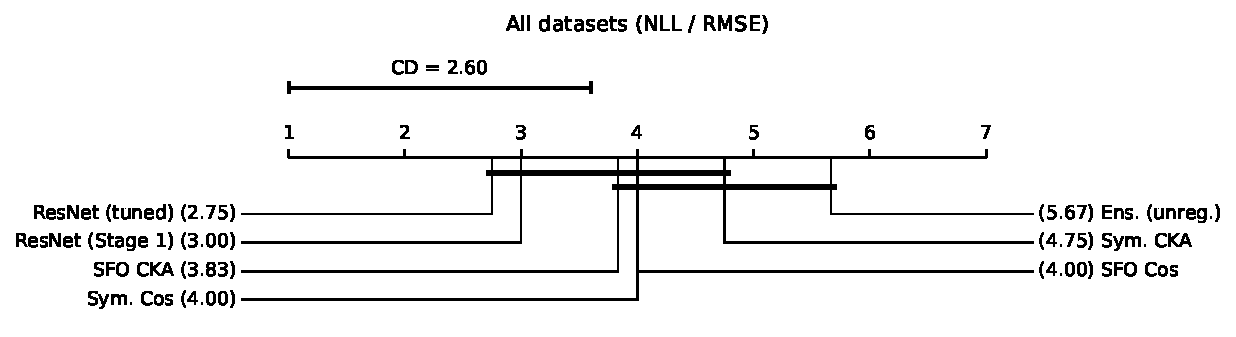
\includegraphics[width=0.75\textwidth]{figures/cd_combined.pdf}
    \caption{Critical difference diagram (Nemenyi, $\alpha = 0.05$) of the mean ranks on all $12$ datasets, ranked by NLL (classification) and RMSE (regression). Methods connected by a bar are not significantly different. The per-task diagrams are shown in Figure~\ref{fig:cd_tasks}.}
    \label{fig:cd}
\end{figure}

\subsection{Ensemble Diagnostics, Stability and Cost}
\label{sec:stability}
Table~\ref{tab:ensemble_diagnostics} and Figure~\ref{fig:staged_loss} summarize the staged loss and the member similarity of the ensembles. Stability, cost and the selected hyperparameters are reported in Appendix~\ref{app:other}.
\begin{itemize}
    \item \textbf{Staged loss.} The first member alone is at least as good as the full ensemble for every ensemble: $L(1)/L(8) = 0.990$--$1.000$ on classification and $0.979$--$0.990$ on regression. On regression the staged loss never decreases with $m$. The first member alone is within about $1\%$ of ResNet (Stage 1) for every ensemble on regression and for all except Sym.\ CKA ($1.8\%$) and Sym.\ Cos ($6.9\%$) on classification.
    \item \textbf{Member contributions.} After scaling by $\nu$, every member $m \ge 2$ contributes at most $6\%$ of the first member's output norm (Figure~\ref{fig:member_norms}).
    \item \textbf{Member similarity.} The mean off-diagonal CKA is $0.612$ for Ens.\ (unreg.), $0.037$ for Sym.\ CKA and $0.060$ for SFO CKA, while the cosine-penalized ensembles keep a high CKA ($0.395$--$0.468$; Figure~\ref{fig:similarity}).
    \item \textbf{Stability.} Every ensemble has a higher seed standard deviation than ResNet (Stage 1) in both tasks (ratio $1.020$--$1.817$, Table~\ref{tab:stability}).
    \item \textbf{Cost.} Every ensemble has $8$ times the parameters of the single ResNet, is refit for fewer epochs (geometric-mean ratio $0.77$--$0.94$) and takes $3.8$--$5.2$ times longer to train (Table~\ref{tab:cost}).
    \item \textbf{Selected penalty weight.} For every regularized ensemble, the selected $\lambda$ spans almost the whole search range, from about $10^{-3}$ to $7.3$--$9.7$ (Figure~\ref{fig:hyperparameters}).
\end{itemize}

\begin{table}[htbp]
    \centering
    \caption{Ensemble diagnostics. Staged loss of the first $m$ members relative to the full ensemble of $M = 8$ (NLL for classification, RMSE for regression; geometric mean over runs and datasets), and the mean off-diagonal pairwise CKA and squared cosine similarity of the members' penultimate representations on the outer test fold (mean over all runs).}
    \label{tab:ensemble_diagnostics}
    \resizebox{\ifdim\width>\textwidth\textwidth\else\width\fi}{!}{%
    \begin{tabular}{lcccccc}
        \toprule
        \textbf{Method} & \multicolumn{2}{c}{\textbf{Classification}} & \multicolumn{2}{c}{\textbf{Regression}} & \multicolumn{2}{c}{\textbf{Similarity}} \\ \cmidrule(lr){2-3} \cmidrule(lr){4-5} \cmidrule(lr){6-7} & $L(1)/L(8)$ & $L(4)/L(8)$ & $L(1)/L(8)$ & $L(4)/L(8)$ & CKA & Cosine \\
        \midrule
        Ens. (unreg.) & 0.992 & 0.994 & 0.979 & 0.989 & 0.612 & 0.101 \\
        Sym. CKA & 1.000 & 0.997 & 0.990 & 0.993 & 0.037 & 0.021 \\
        Sym. Cos & 0.991 & 0.992 & 0.982 & 0.989 & 0.468 & 0.018 \\
        SFO CKA & 1.000 & 0.996 & 0.984 & 0.991 & 0.060 & 0.021 \\
        SFO Cos & 0.990 & 0.991 & 0.982 & 0.990 & 0.395 & 0.021 \\
        \bottomrule
    \end{tabular}%
    }
\end{table}


\begin{figure}[htbp]
    \centering
    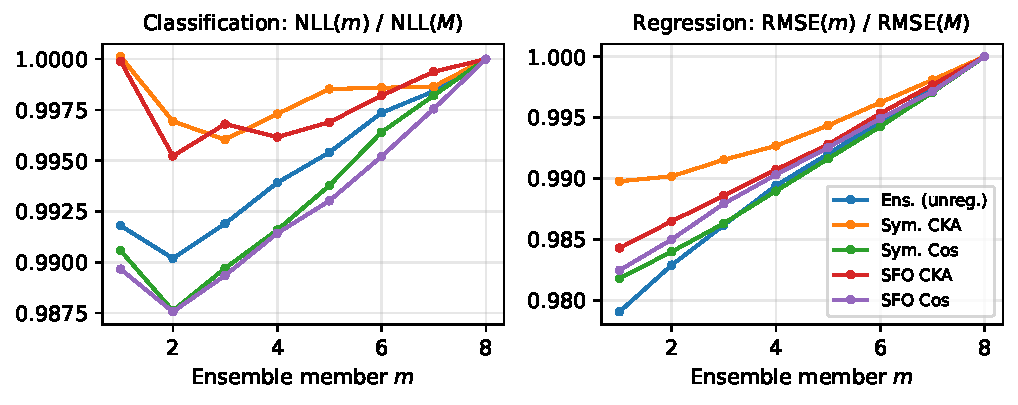
\includegraphics[width=0.9\textwidth]{figures/staged_loss.pdf}
    \caption{Staged loss of the first $m$ members, $\hat{Y}^{(m)} = f_1(X) + \nu \sum_{j=2}^{m} f_j(X)$, relative to the full ensemble ($M = 8$). Geometric mean over the $25$ runs of each dataset and then over the $6$ datasets of each task.}
    \label{fig:staged_loss}
\end{figure}

\section{Conclusions and Discussion}

\subsection{Key Findings}
\begin{itemize}
    \item \textbf{Single ResNets beat ensembles} They have the two best mean ranks in every metric ($1.92$ and $2.25$ over all $12$ datasets, Table~\ref{tab:mean_ranks}), and the Friedman test rejects the equality of the methods for every metric (Table~\ref{tab:friedman}). No ensemble is significantly better than either single ResNet in any test.
    \item \textbf{The differences are significant in rank but small in magnitude.} The ranking of the methods is consistent across datasets, but the geometric-mean loss ratios of the ensembles exceed those of ResNet (Stage 1) by only $0.6$--$4.3\%$, with the exception of Sym.\ Cos on classification NLL ($8\%$, Table~\ref{tab:gm_loss_ratios}). Accuracy and ROC-AUC differ by less than $0.9\%$ on all classification datasets except MiniBooNE. The per-task Wilcoxon tests find no significant difference after the Holm correction, and the few significant differences in the loss values (e.g.\ NLL on Covertype, SFO CKA vs.\ ResNet (tuned) on the combined ratios) all favour the single ResNets.
    \item \textbf{The SFO CKA model is the best ensemble.} A CKA-penalized ensemble has the best ensemble rank in every metric, and SFO CKA is significantly better than Sym.\ Cos over all $12$ datasets. The penalties do decorrelate the members (mean CKA $0.037$--$0.060$ vs.\ $0.612$ without a penalty, Table~\ref{tab:ensemble_diagnostics}), but this does not translate into a lower loss than that of a single network.
    \item \textbf{Adding members does not help.} The first member alone is at least as good as the full ensemble ($L(1)/L(8) \le 1$ for every ensemble), and every member $m \ge 2$ contributes at most $6\%$ of the first member's output norm. At the same time, the ensembles are less stable across seeds ($\bar{\sigma}_{\text{seed}}$ ratio $1.020$--$1.817$, Section~\ref{sec:stability}) and take $3.8$--$5.2$ times longer to train (Table~\ref{tab:cost}).
\end{itemize}

\subsection{Explanation of Failures}
\begin{itemize}
    \item \textbf{A strong first learner leaves no room for the other members.} A tuned Tabular ResNet already performs close to the best achievable level on these datasets: the first member of every ensemble is, on its own, within about $1\%$ of ResNet (Stage 1) on regression and on most classification ensembles. What remains for members $2$ to $8$ is a small residual of the \emph{training} data that consists mostly of noise. Fitting it does not generalize, so the later members stay small, are further shrunk by $\nu$, and at best do not change the prediction.
    \item \textbf{Simultaneous training of the members is disruptive.} In our interpretation, the parallel form of dynamic boosting is the an important reason why the later members add nothing, in line with the observation that joint training of deep ensembles leads to learner collusion~\cite{jeffares2023joint}:
    \begin{itemize}
        \item the target of every member $m \ge 2$ is the residual of predecessors that are themselves still changing, so it is a moving target until the end of training;
        \item all members share one training length, chosen on the validation loss of the whole ensemble, and the ensembles are refit for fewer epochs than the single ResNet (ratio $0.77$--$0.94$), so the first member is trained for less time than a standalone network;
        \item the higher seed standard deviation of all ensembles and the staged classification loss, which increases from $m = 2$ to $m = 8$, are consistent with this.
    \end{itemize}
    We therefore consider simultaneous training unsuitable for additive ensembles of strong networks; 
\end{itemize}

\subsection{Limitations}
\begin{itemize}
    \item Only $12$ of the planned $24$ datasets were used, which limits the power of the between-dataset tests: with $N = 6$ datasets per task, the smallest attainable Wilcoxon $p$-value ($0.031$) cannot survive the Holm correction.
    \item Hyperparameters were selected on a single $80/20$ inner split, which makes the selection noisy, as the wide spread of the selected $\lambda$ values shows (Figure~\ref{fig:hyperparameters}).
    \item The budgets are not matched: every ensemble has $8$ times the parameters of the single ResNet and needs $3.8$--$5.2$ times its training time, while the tuning budget (number of trials) is the same.
    \item Losses are reported in the units of each dataset, so their magnitudes cannot be pooled across datasets; the cross-dataset comparison relies on ranks and ratios.
    \item Tested datasets were to small for proposed architectures which fully exploited their potential leaving no room for possible ensemble improvement
    \item Ensemble methods having more hyperparameters consume more compute for tuning with comparable accuracy
\end{itemize}

\subsection{Future Work}
\begin{enumerate}
    \item \textbf{Sequential boosting.} Member $m$ would be trained only after members $1, \dots, m-1$ are frozen, so that its residual target is fixed. This also allows a separate early stopping for each member and weaker (smaller) members after the first.
    \item \textbf{Compute-matched comparison.} The number of training FLOPs of the single ResNet would be recorded, including the whole hyperparameter search (all trials, including pruned ones), as the forward and backward FLOPs per sample times the number of samples and epochs. Each ensemble, again including its hyperparameter search, would then receive a comparable budget, with a tolerance (e.g.\ $\pm 3\%$) that lets a running epoch or trial finish. Two variants are of interest:
    \begin{enumerate}
        \item the single ResNet is trained as in this study, until the maximum number of epochs or the early-stopping patience is reached;
        \item the single ResNet is deliberately stopped early (e.g.\ at an accuracy of about $0.7$ of accuracy of a fully trained or after a fixed fraction of its budget), and the ensemble receives the same reduced budget, which gives it room to exploit many weak learners.
    \end{enumerate}
    The second variant is artificial as an experiment, but it simulates the practically relevant setting in which computational resources are limited.
    \item \textbf{Standardized statistics.} The magnitudes of losses such as RMSE and MAE depend heavily on the dataset. Normalizing them, e.g.\ by the standard deviation of the target, or using standardized per-dataset effect sizes would allow magnitude-based tests that pool all datasets instead of relying on ranks only.
    \item \textbf{Training-set size.} Ensembles mainly reduce variance, which matters most when data is scarce. Subsampling the training partitions to about $1{,}000$ and $5{,}000$ rows on $4$--$6$ datasets would show whether the ensembles overtake the single ResNet at small sizes.
    \item \textbf{Metrics where ensembles usually help.} Calibration (e.g.\ expected calibration error), the quality of uncertainty estimates derived from the disagreement of the members, and robustness to noisy or missing features at test time.
    \item \textbf{A less noisy comparison.} Repeated inner validation and the full set of $24$ datasets to increase the power of the statistical tests.
\end{enumerate}

\section{Reproducibility}

\subsection{Reproducibility}
% Ported from initial_plan.tex.
To guarantee full experimental reproducibility across hardware environments, the project will enforce strict determinism and standardized code distribution:

\begin{enumerate}
    \item \textbf{Deterministic Random Seeding:} All sources of stochasticity—including dataset cross-validation partitioning, weight initialization, dropout masks, mini-batch shuffling, and Bayesian hyperparameter sampling—will be controlled using fixed integer seeds:
    \begin{itemize}
        \item Cross-validation splits (\texttt{StratifiedKFold} and \texttt{KFold} in \texttt{scikit-learn}) and \texttt{Optuna}'s \texttt{TPESampler} will be initialized with a fixed master seed ($s_{\text{master}} = 42$).
        \item For the $S = 5$ repeated evaluation runs per fold, all random number generators (\texttt{python.random}, \texttt{numpy.random}, \texttt{torch.manual\_seed}, and \texttt{torch.cuda.manual\_seed\_all}) will be explicitly initialized with the fixed seed set $\mathcal{S} = \{42, 67, 69, 228, 2137\}$.
        \item Within each $M$-model ensemble run initialized with global seed $s \in \mathcal{S}$, individual member networks $f_m$ ($m \in \{1, \dots, M\}$) will be initialized deterministically using derived sub-seeds $s_m = 1000 s + m$ so that starting weights are distinct across learners yet strictly reproducible across runs.
        \item PyTorch deterministic execution flags (\texttt{torch.backends.cudnn.deterministic = True} and \texttt{torch.backends.cudnn.benchmark = False}) will be enabled during training and evaluation.
    \end{itemize}
    \item \textbf{Public Repository and Execution Instructions:} All source code, preprocessing pipelines, tuned hyperparameter configuration files, and statistical analysis scripts will be maintained in a public GitHub repository (and included in the final LeON submission archive). The repository will contain:
    \begin{itemize}
        \item A pinned environment specification (\texttt{requirements.txt} and \texttt{environment.yml}) locking exact versions of Python, PyTorch, CUDA, \texttt{scikit-learn}, \texttt{openml}, and \texttt{optuna}.
        \item Automated data-fetching scripts that download and cache the $24$ OpenML datasets via their exact dataset IDs (Tables~\ref{tab:clf_datasets} and~\ref{tab:reg_datasets}).
        \item A step-by-step \texttt{README.md} documenting the exact command-line instructions required to reproduce hyperparameter tuning, model training, metric aggregation, and figure/table generation from scratch.
    \end{itemize}
\end{enumerate}


\section{External Code and AI Usage Disclosure}
% Ported from initial_plan.tex.
\paragraph{Planned Use and Modification of External Code.}
In accordance with course guidelines, any external code utilized for baselines or data loading will be explicitly cited in the final report and substantially modified to fit our experimental pipeline:
\begin{itemize}
    \item \textbf{Data Loading and Tabular ResNet Reference:} We will adapt dataset loading utilities and reference Tabular ResNet block definitions from the open-source Inria Tabular Benchmark repository (\texttt{LeoGrin/tabular-benchmark}) \cite{grinsztajn2022why}, modifying the architecture to expose penultimate batch-centered latent representations $\tilde{Z}_m$ and support simultaneous multi-model forward passes.
    \item \textbf{TANGOS Baseline:} We will adapt the intra-model gradient orthogonalization loss calculation from the official Cambridge repository (\texttt{vanderschaarlab/TANGOS}) \cite{jeffares2023tangos}, integrating it into our unified Tabular ResNet training loop.
    \item \textbf{Original Implementation:} The core contributions of this project—specifically the additive multi-network ensemble wrapper, the lower-triangular stop-gradient mask ($\text{SFOvTSGM}$), and the vectorized $\Phi_{\text{CKA}}$ and $\Phi_{\text{Cos}}$ repulsion loss modules—will be implemented from scratch in PyTorch.
\end{itemize}

\paragraph{AI Usage Disclosure.}
In compliance with the course policy on artificial intelligence disclosure, the authors declare that the text, mathematical typesetting, and LaTeX structure of this Project Plan (spanning Sections~1 through~7 and the accompanying BibTeX bibliography) were generated in their entirety by a Large Language Model (AI assistant). 

This generation process was conducted under continuous, substantial human supervision and direction.


% ==========================================
% REFERENCES
% ==========================================
\newpage
\bibliographystyle{plain}
\bibliography{bibliography}

% ==========================================
% APPENDIX
% ==========================================
\appendix

% ==========================================
% APPENDIX
% ==========================================
\appendix

\section{Additional Results}
\label{app:results}

\subsection{Secondary Metrics}
Tables~\ref{tab:results_accuracy}--\ref{tab:results_r2} report the secondary metrics on every dataset.

\begin{table}[htbp]
    \centering
    \small
    \setlength{\tabcolsep}{4pt}
    \caption{Classification: outer-test Accuracy (higher is better), mean $\pm$ standard deviation over 5 outer folds $\times$ 5 seeds. Best mean in bold; $^{\uparrow}$/$^{\downarrow}$: significantly better/worse than Ens. (unreg.) (paired $t$-test over fold means, $p < 0.05$).}
    \label{tab:results_accuracy}
    \resizebox{\ifdim\width>\textwidth\textwidth\else\width\fi}{!}{%
    \begin{tabular}{lccccccc}
        \toprule
        \textbf{Dataset} & \textbf{\begin{tabular}[t]{@{}c@{}}ResNet\\(Stage 1)\end{tabular}} & \textbf{\begin{tabular}[t]{@{}c@{}}ResNet\\(tuned)\end{tabular}} & \textbf{\begin{tabular}[t]{@{}c@{}}Ens.\\(unreg.)\end{tabular}} & \textbf{\begin{tabular}[t]{@{}c@{}}Sym.\\CKA\end{tabular}} & \textbf{\begin{tabular}[t]{@{}c@{}}Sym.\\Cos\end{tabular}} & \textbf{\begin{tabular}[t]{@{}c@{}}SFO\\CKA\end{tabular}} & \textbf{\begin{tabular}[t]{@{}c@{}}SFO\\Cos\end{tabular}} \\
        \midrule
        Electricity & \begin{tabular}[t]{@{}c@{}}0.8446\\{\scriptsize $\pm$0.0060}\end{tabular} & \begin{tabular}[t]{@{}c@{}}\textbf{0.8451}\\{\scriptsize $\pm$0.0049}\end{tabular} & \begin{tabular}[t]{@{}c@{}}0.8409\\{\scriptsize $\pm$0.0043}\end{tabular} & \begin{tabular}[t]{@{}c@{}}0.8407\\{\scriptsize $\pm$0.0057}\end{tabular} & \begin{tabular}[t]{@{}c@{}}0.8394\\{\scriptsize $\pm$0.0052}\end{tabular} & \begin{tabular}[t]{@{}c@{}}0.8426\\{\scriptsize $\pm$0.0065}\end{tabular} & \begin{tabular}[t]{@{}c@{}}0.8407\\{\scriptsize $\pm$0.0057}\end{tabular} \\
        Credit & \begin{tabular}[t]{@{}c@{}}0.7509$^{\uparrow}$\\{\scriptsize $\pm$0.0096}\end{tabular} & \begin{tabular}[t]{@{}c@{}}0.7508$^{\uparrow}$\\{\scriptsize $\pm$0.0101}\end{tabular} & \begin{tabular}[t]{@{}c@{}}0.7470\\{\scriptsize $\pm$0.0102}\end{tabular} & \begin{tabular}[t]{@{}c@{}}0.7505\\{\scriptsize $\pm$0.0097}\end{tabular} & \begin{tabular}[t]{@{}c@{}}0.7504\\{\scriptsize $\pm$0.0081}\end{tabular} & \begin{tabular}[t]{@{}c@{}}\textbf{0.7510}$^{\uparrow}$\\{\scriptsize $\pm$0.0096}\end{tabular} & \begin{tabular}[t]{@{}c@{}}0.7501$^{\uparrow}$\\{\scriptsize $\pm$0.0089}\end{tabular} \\
        Default Credit Card & \begin{tabular}[t]{@{}c@{}}0.7100\\{\scriptsize $\pm$0.0101}\end{tabular} & \begin{tabular}[t]{@{}c@{}}0.7098\\{\scriptsize $\pm$0.0102}\end{tabular} & \begin{tabular}[t]{@{}c@{}}0.7088\\{\scriptsize $\pm$0.0113}\end{tabular} & \begin{tabular}[t]{@{}c@{}}\textbf{0.7110}\\{\scriptsize $\pm$0.0074}\end{tabular} & \begin{tabular}[t]{@{}c@{}}0.7077\\{\scriptsize $\pm$0.0109}\end{tabular} & \begin{tabular}[t]{@{}c@{}}0.7093\\{\scriptsize $\pm$0.0087}\end{tabular} & \begin{tabular}[t]{@{}c@{}}0.7089\\{\scriptsize $\pm$0.0099}\end{tabular} \\
        Covertype & \begin{tabular}[t]{@{}c@{}}0.9130$^{\uparrow}$\\{\scriptsize $\pm$0.0022}\end{tabular} & \begin{tabular}[t]{@{}c@{}}\textbf{0.9136}$^{\uparrow}$\\{\scriptsize $\pm$0.0024}\end{tabular} & \begin{tabular}[t]{@{}c@{}}0.9056\\{\scriptsize $\pm$0.0050}\end{tabular} & \begin{tabular}[t]{@{}c@{}}0.9066\\{\scriptsize $\pm$0.0058}\end{tabular} & \begin{tabular}[t]{@{}c@{}}0.9063\\{\scriptsize $\pm$0.0065}\end{tabular} & \begin{tabular}[t]{@{}c@{}}0.9085\\{\scriptsize $\pm$0.0054}\end{tabular} & \begin{tabular}[t]{@{}c@{}}0.9068\\{\scriptsize $\pm$0.0038}\end{tabular} \\
        Pol & \begin{tabular}[t]{@{}c@{}}0.9853\\{\scriptsize $\pm$0.0018}\end{tabular} & \begin{tabular}[t]{@{}c@{}}0.9850\\{\scriptsize $\pm$0.0028}\end{tabular} & \begin{tabular}[t]{@{}c@{}}\textbf{0.9853}\\{\scriptsize $\pm$0.0047}\end{tabular} & \begin{tabular}[t]{@{}c@{}}0.9851\\{\scriptsize $\pm$0.0036}\end{tabular} & \begin{tabular}[t]{@{}c@{}}0.9838\\{\scriptsize $\pm$0.0046}\end{tabular} & \begin{tabular}[t]{@{}c@{}}0.9847\\{\scriptsize $\pm$0.0043}\end{tabular} & \begin{tabular}[t]{@{}c@{}}0.9836\\{\scriptsize $\pm$0.0042}\end{tabular} \\
        MiniBooNE & \begin{tabular}[t]{@{}c@{}}0.9163\\{\scriptsize $\pm$0.0307}\end{tabular} & \begin{tabular}[t]{@{}c@{}}0.9308$^{\uparrow}$\\{\scriptsize $\pm$0.0127}\end{tabular} & \begin{tabular}[t]{@{}c@{}}0.9286\\{\scriptsize $\pm$0.0162}\end{tabular} & \begin{tabular}[t]{@{}c@{}}0.9159\\{\scriptsize $\pm$0.0407}\end{tabular} & \begin{tabular}[t]{@{}c@{}}0.8804\\{\scriptsize $\pm$0.0906}\end{tabular} & \begin{tabular}[t]{@{}c@{}}0.9263\\{\scriptsize $\pm$0.0142}\end{tabular} & \begin{tabular}[t]{@{}c@{}}\textbf{0.9336}\\{\scriptsize $\pm$0.0026}\end{tabular} \\
        \bottomrule
    \end{tabular}%
    }
\end{table}

\begin{table}[htbp]
    \centering
    \small
    \setlength{\tabcolsep}{4pt}
    \caption{Classification: outer-test ROC-AUC (higher is better), mean $\pm$ standard deviation over 5 outer folds $\times$ 5 seeds. Best mean in bold; $^{\uparrow}$/$^{\downarrow}$: significantly better/worse than Ens. (unreg.) (paired $t$-test over fold means, $p < 0.05$).}
    \label{tab:results_roc_auc}
    \resizebox{\ifdim\width>\textwidth\textwidth\else\width\fi}{!}{%
    \begin{tabular}{lccccccc}
        \toprule
        \textbf{Dataset} & \textbf{\begin{tabular}[t]{@{}c@{}}ResNet\\(Stage 1)\end{tabular}} & \textbf{\begin{tabular}[t]{@{}c@{}}ResNet\\(tuned)\end{tabular}} & \textbf{\begin{tabular}[t]{@{}c@{}}Ens.\\(unreg.)\end{tabular}} & \textbf{\begin{tabular}[t]{@{}c@{}}Sym.\\CKA\end{tabular}} & \textbf{\begin{tabular}[t]{@{}c@{}}Sym.\\Cos\end{tabular}} & \textbf{\begin{tabular}[t]{@{}c@{}}SFO\\CKA\end{tabular}} & \textbf{\begin{tabular}[t]{@{}c@{}}SFO\\Cos\end{tabular}} \\
        \midrule
        Electricity & \begin{tabular}[t]{@{}c@{}}0.9259$^{\uparrow}$\\{\scriptsize $\pm$0.0035}\end{tabular} & \begin{tabular}[t]{@{}c@{}}\textbf{0.9269}$^{\uparrow}$\\{\scriptsize $\pm$0.0024}\end{tabular} & \begin{tabular}[t]{@{}c@{}}0.9220\\{\scriptsize $\pm$0.0035}\end{tabular} & \begin{tabular}[t]{@{}c@{}}0.9226\\{\scriptsize $\pm$0.0037}\end{tabular} & \begin{tabular}[t]{@{}c@{}}0.9236\\{\scriptsize $\pm$0.0031}\end{tabular} & \begin{tabular}[t]{@{}c@{}}0.9222\\{\scriptsize $\pm$0.0033}\end{tabular} & \begin{tabular}[t]{@{}c@{}}0.9229\\{\scriptsize $\pm$0.0039}\end{tabular} \\
        Credit & \begin{tabular}[t]{@{}c@{}}0.8232$^{\uparrow}$\\{\scriptsize $\pm$0.0104}\end{tabular} & \begin{tabular}[t]{@{}c@{}}\textbf{0.8239}$^{\uparrow}$\\{\scriptsize $\pm$0.0110}\end{tabular} & \begin{tabular}[t]{@{}c@{}}0.8216\\{\scriptsize $\pm$0.0109}\end{tabular} & \begin{tabular}[t]{@{}c@{}}0.8220\\{\scriptsize $\pm$0.0100}\end{tabular} & \begin{tabular}[t]{@{}c@{}}0.8221\\{\scriptsize $\pm$0.0106}\end{tabular} & \begin{tabular}[t]{@{}c@{}}0.8231\\{\scriptsize $\pm$0.0095}\end{tabular} & \begin{tabular}[t]{@{}c@{}}0.8221\\{\scriptsize $\pm$0.0097}\end{tabular} \\
        Default Credit Card & \begin{tabular}[t]{@{}c@{}}\textbf{0.7771}\\{\scriptsize $\pm$0.0091}\end{tabular} & \begin{tabular}[t]{@{}c@{}}0.7757\\{\scriptsize $\pm$0.0091}\end{tabular} & \begin{tabular}[t]{@{}c@{}}0.7755\\{\scriptsize $\pm$0.0097}\end{tabular} & \begin{tabular}[t]{@{}c@{}}0.7753\\{\scriptsize $\pm$0.0095}\end{tabular} & \begin{tabular}[t]{@{}c@{}}0.7760\\{\scriptsize $\pm$0.0103}\end{tabular} & \begin{tabular}[t]{@{}c@{}}0.7737\\{\scriptsize $\pm$0.0105}\end{tabular} & \begin{tabular}[t]{@{}c@{}}0.7751\\{\scriptsize $\pm$0.0102}\end{tabular} \\
        Covertype & \begin{tabular}[t]{@{}c@{}}0.9733$^{\uparrow}$\\{\scriptsize $\pm$0.0012}\end{tabular} & \begin{tabular}[t]{@{}c@{}}\textbf{0.9736}$^{\uparrow}$\\{\scriptsize $\pm$0.0010}\end{tabular} & \begin{tabular}[t]{@{}c@{}}0.9696\\{\scriptsize $\pm$0.0016}\end{tabular} & \begin{tabular}[t]{@{}c@{}}0.9712\\{\scriptsize $\pm$0.0028}\end{tabular} & \begin{tabular}[t]{@{}c@{}}0.9706\\{\scriptsize $\pm$0.0013}\end{tabular} & \begin{tabular}[t]{@{}c@{}}0.9710\\{\scriptsize $\pm$0.0020}\end{tabular} & \begin{tabular}[t]{@{}c@{}}0.9710\\{\scriptsize $\pm$0.0011}\end{tabular} \\
        Pol & \begin{tabular}[t]{@{}c@{}}0.9993\\{\scriptsize $\pm$0.0001}\end{tabular} & \begin{tabular}[t]{@{}c@{}}0.9993\\{\scriptsize $\pm$0.0002}\end{tabular} & \begin{tabular}[t]{@{}c@{}}\textbf{0.9993}\\{\scriptsize $\pm$0.0002}\end{tabular} & \begin{tabular}[t]{@{}c@{}}0.9992$^{\downarrow}$\\{\scriptsize $\pm$0.0002}\end{tabular} & \begin{tabular}[t]{@{}c@{}}0.9992\\{\scriptsize $\pm$0.0003}\end{tabular} & \begin{tabular}[t]{@{}c@{}}0.9992\\{\scriptsize $\pm$0.0002}\end{tabular} & \begin{tabular}[t]{@{}c@{}}0.9992\\{\scriptsize $\pm$0.0002}\end{tabular} \\
        MiniBooNE & \begin{tabular}[t]{@{}c@{}}0.9792\\{\scriptsize $\pm$0.0023}\end{tabular} & \begin{tabular}[t]{@{}c@{}}\textbf{0.9803}\\{\scriptsize $\pm$0.0030}\end{tabular} & \begin{tabular}[t]{@{}c@{}}0.9788\\{\scriptsize $\pm$0.0023}\end{tabular} & \begin{tabular}[t]{@{}c@{}}0.9792\\{\scriptsize $\pm$0.0022}\end{tabular} & \begin{tabular}[t]{@{}c@{}}0.9783\\{\scriptsize $\pm$0.0032}\end{tabular} & \begin{tabular}[t]{@{}c@{}}0.9768\\{\scriptsize $\pm$0.0056}\end{tabular} & \begin{tabular}[t]{@{}c@{}}0.9781\\{\scriptsize $\pm$0.0049}\end{tabular} \\
        \bottomrule
    \end{tabular}%
    }
\end{table}

\begin{table}[htbp]
    \centering
    \small
    \setlength{\tabcolsep}{4pt}
    \caption{Regression: outer-test MAE (lower is better), mean $\pm$ standard deviation over 5 outer folds $\times$ 5 seeds. Best mean in bold; $^{\uparrow}$/$^{\downarrow}$: significantly better/worse than Ens. (unreg.) (paired $t$-test over fold means, $p < 0.05$).}
    \label{tab:results_mae}
    \resizebox{\ifdim\width>\textwidth\textwidth\else\width\fi}{!}{%
    \begin{tabular}{lccccccc}
        \toprule
        \textbf{Dataset} & \textbf{\begin{tabular}[t]{@{}c@{}}ResNet\\(Stage 1)\end{tabular}} & \textbf{\begin{tabular}[t]{@{}c@{}}ResNet\\(tuned)\end{tabular}} & \textbf{\begin{tabular}[t]{@{}c@{}}Ens.\\(unreg.)\end{tabular}} & \textbf{\begin{tabular}[t]{@{}c@{}}Sym.\\CKA\end{tabular}} & \textbf{\begin{tabular}[t]{@{}c@{}}Sym.\\Cos\end{tabular}} & \textbf{\begin{tabular}[t]{@{}c@{}}SFO\\CKA\end{tabular}} & \textbf{\begin{tabular}[t]{@{}c@{}}SFO\\Cos\end{tabular}} \\
        \midrule
        California Housing & \begin{tabular}[t]{@{}c@{}}0.1081\\{\scriptsize $\pm$0.0040}\end{tabular} & \begin{tabular}[t]{@{}c@{}}0.1069\\{\scriptsize $\pm$0.0041}\end{tabular} & \begin{tabular}[t]{@{}c@{}}0.1083\\{\scriptsize $\pm$0.0035}\end{tabular} & \begin{tabular}[t]{@{}c@{}}0.1075\\{\scriptsize $\pm$0.0040}\end{tabular} & \begin{tabular}[t]{@{}c@{}}0.1062\\{\scriptsize $\pm$0.0031}\end{tabular} & \begin{tabular}[t]{@{}c@{}}\textbf{0.1058}\\{\scriptsize $\pm$0.0034}\end{tabular} & \begin{tabular}[t]{@{}c@{}}0.1066\\{\scriptsize $\pm$0.0034}\end{tabular} \\
        House 16H & \begin{tabular}[t]{@{}c@{}}0.3145\\{\scriptsize $\pm$0.0118}\end{tabular} & \begin{tabular}[t]{@{}c@{}}0.3168\\{\scriptsize $\pm$0.0083}\end{tabular} & \begin{tabular}[t]{@{}c@{}}0.3170\\{\scriptsize $\pm$0.0111}\end{tabular} & \begin{tabular}[t]{@{}c@{}}0.3223\\{\scriptsize $\pm$0.0105}\end{tabular} & \begin{tabular}[t]{@{}c@{}}0.3210\\{\scriptsize $\pm$0.0132}\end{tabular} & \begin{tabular}[t]{@{}c@{}}\textbf{0.3136}\\{\scriptsize $\pm$0.0133}\end{tabular} & \begin{tabular}[t]{@{}c@{}}0.3180\\{\scriptsize $\pm$0.0124}\end{tabular} \\
        Diamonds & \begin{tabular}[t]{@{}c@{}}0.0679\\{\scriptsize $\pm$0.0043}\end{tabular} & \begin{tabular}[t]{@{}c@{}}0.0719\\{\scriptsize $\pm$0.0074}\end{tabular} & \begin{tabular}[t]{@{}c@{}}0.0693\\{\scriptsize $\pm$0.0069}\end{tabular} & \begin{tabular}[t]{@{}c@{}}0.0679\\{\scriptsize $\pm$0.0052}\end{tabular} & \begin{tabular}[t]{@{}c@{}}\textbf{0.0666}$^{\uparrow}$\\{\scriptsize $\pm$0.0029}\end{tabular} & \begin{tabular}[t]{@{}c@{}}0.0702\\{\scriptsize $\pm$0.0064}\end{tabular} & \begin{tabular}[t]{@{}c@{}}0.0689\\{\scriptsize $\pm$0.0051}\end{tabular} \\
        Elevators ($\times 10^{-3}$) & \begin{tabular}[t]{@{}c@{}}1.400$^{\uparrow}$\\{\scriptsize $\pm$0.024}\end{tabular} & \begin{tabular}[t]{@{}c@{}}1.403\\{\scriptsize $\pm$0.025}\end{tabular} & \begin{tabular}[t]{@{}c@{}}1.414\\{\scriptsize $\pm$0.032}\end{tabular} & \begin{tabular}[t]{@{}c@{}}1.414\\{\scriptsize $\pm$0.026}\end{tabular} & \begin{tabular}[t]{@{}c@{}}\textbf{1.398}$^{\uparrow}$\\{\scriptsize $\pm$0.023}\end{tabular} & \begin{tabular}[t]{@{}c@{}}1.400$^{\uparrow}$\\{\scriptsize $\pm$0.025}\end{tabular} & \begin{tabular}[t]{@{}c@{}}1.403\\{\scriptsize $\pm$0.032}\end{tabular} \\
        Ailerons ($\times 10^{-4}$) & \begin{tabular}[t]{@{}c@{}}\textbf{1.159}\\{\scriptsize $\pm$0.019}\end{tabular} & \begin{tabular}[t]{@{}c@{}}1.163\\{\scriptsize $\pm$0.019}\end{tabular} & \begin{tabular}[t]{@{}c@{}}1.165\\{\scriptsize $\pm$0.017}\end{tabular} & \begin{tabular}[t]{@{}c@{}}1.174\\{\scriptsize $\pm$0.024}\end{tabular} & \begin{tabular}[t]{@{}c@{}}1.166\\{\scriptsize $\pm$0.022}\end{tabular} & \begin{tabular}[t]{@{}c@{}}1.166\\{\scriptsize $\pm$0.024}\end{tabular} & \begin{tabular}[t]{@{}c@{}}1.169\\{\scriptsize $\pm$0.025}\end{tabular} \\
        Bike Sharing Demand & \begin{tabular}[t]{@{}c@{}}32.40\\{\scriptsize $\pm$3.33}\end{tabular} & \begin{tabular}[t]{@{}c@{}}30.25\\{\scriptsize $\pm$2.12}\end{tabular} & \begin{tabular}[t]{@{}c@{}}31.96\\{\scriptsize $\pm$3.15}\end{tabular} & \begin{tabular}[t]{@{}c@{}}30.57\\{\scriptsize $\pm$2.23}\end{tabular} & \begin{tabular}[t]{@{}c@{}}30.72\\{\scriptsize $\pm$2.53}\end{tabular} & \begin{tabular}[t]{@{}c@{}}\textbf{29.87}\\{\scriptsize $\pm$1.37}\end{tabular} & \begin{tabular}[t]{@{}c@{}}30.16\\{\scriptsize $\pm$2.62}\end{tabular} \\
        \bottomrule
    \end{tabular}%
    }
\end{table}

\begin{table}[htbp]
    \centering
    \small
    \setlength{\tabcolsep}{4pt}
    \caption{Regression: outer-test $R^2$ (higher is better), mean $\pm$ standard deviation over 5 outer folds $\times$ 5 seeds. Best mean in bold; $^{\uparrow}$/$^{\downarrow}$: significantly better/worse than Ens. (unreg.) (paired $t$-test over fold means, $p < 0.05$).}
    \label{tab:results_r2}
    \resizebox{\ifdim\width>\textwidth\textwidth\else\width\fi}{!}{%
    \begin{tabular}{lccccccc}
        \toprule
        \textbf{Dataset} & \textbf{\begin{tabular}[t]{@{}c@{}}ResNet\\(Stage 1)\end{tabular}} & \textbf{\begin{tabular}[t]{@{}c@{}}ResNet\\(tuned)\end{tabular}} & \textbf{\begin{tabular}[t]{@{}c@{}}Ens.\\(unreg.)\end{tabular}} & \textbf{\begin{tabular}[t]{@{}c@{}}Sym.\\CKA\end{tabular}} & \textbf{\begin{tabular}[t]{@{}c@{}}Sym.\\Cos\end{tabular}} & \textbf{\begin{tabular}[t]{@{}c@{}}SFO\\CKA\end{tabular}} & \textbf{\begin{tabular}[t]{@{}c@{}}SFO\\Cos\end{tabular}} \\
        \midrule
        California Housing & \begin{tabular}[t]{@{}c@{}}0.8033\\{\scriptsize $\pm$0.0265}\end{tabular} & \begin{tabular}[t]{@{}c@{}}0.8107\\{\scriptsize $\pm$0.0300}\end{tabular} & \begin{tabular}[t]{@{}c@{}}0.7709\\{\scriptsize $\pm$0.1761}\end{tabular} & \begin{tabular}[t]{@{}c@{}}0.8108\\{\scriptsize $\pm$0.0142}\end{tabular} & \begin{tabular}[t]{@{}c@{}}0.8011\\{\scriptsize $\pm$0.0575}\end{tabular} & \begin{tabular}[t]{@{}c@{}}\textbf{0.8132}\\{\scriptsize $\pm$0.0179}\end{tabular} & \begin{tabular}[t]{@{}c@{}}0.8063\\{\scriptsize $\pm$0.0431}\end{tabular} \\
        House 16H & \begin{tabular}[t]{@{}c@{}}0.4857\\{\scriptsize $\pm$0.0431}\end{tabular} & \begin{tabular}[t]{@{}c@{}}0.4851\\{\scriptsize $\pm$0.0404}\end{tabular} & \begin{tabular}[t]{@{}c@{}}0.4835\\{\scriptsize $\pm$0.0564}\end{tabular} & \begin{tabular}[t]{@{}c@{}}0.4732\\{\scriptsize $\pm$0.0404}\end{tabular} & \begin{tabular}[t]{@{}c@{}}0.4723\\{\scriptsize $\pm$0.0695}\end{tabular} & \begin{tabular}[t]{@{}c@{}}0.4948\\{\scriptsize $\pm$0.0460}\end{tabular} & \begin{tabular}[t]{@{}c@{}}\textbf{0.4956}\\{\scriptsize $\pm$0.0372}\end{tabular} \\
        Diamonds & \begin{tabular}[t]{@{}c@{}}0.9915\\{\scriptsize $\pm$0.0009}\end{tabular} & \begin{tabular}[t]{@{}c@{}}0.9903\\{\scriptsize $\pm$0.0018}\end{tabular} & \begin{tabular}[t]{@{}c@{}}0.9908\\{\scriptsize $\pm$0.0016}\end{tabular} & \begin{tabular}[t]{@{}c@{}}0.9913\\{\scriptsize $\pm$0.0013}\end{tabular} & \begin{tabular}[t]{@{}c@{}}\textbf{0.9915}\\{\scriptsize $\pm$0.0007}\end{tabular} & \begin{tabular}[t]{@{}c@{}}0.9908\\{\scriptsize $\pm$0.0014}\end{tabular} & \begin{tabular}[t]{@{}c@{}}0.9910\\{\scriptsize $\pm$0.0012}\end{tabular} \\
        Elevators & \begin{tabular}[t]{@{}c@{}}0.9191$^{\uparrow}$\\{\scriptsize $\pm$0.0047}\end{tabular} & \begin{tabular}[t]{@{}c@{}}0.9183\\{\scriptsize $\pm$0.0066}\end{tabular} & \begin{tabular}[t]{@{}c@{}}0.9175\\{\scriptsize $\pm$0.0062}\end{tabular} & \begin{tabular}[t]{@{}c@{}}0.9184\\{\scriptsize $\pm$0.0055}\end{tabular} & \begin{tabular}[t]{@{}c@{}}\textbf{0.9201}$^{\uparrow}$\\{\scriptsize $\pm$0.0048}\end{tabular} & \begin{tabular}[t]{@{}c@{}}0.9187\\{\scriptsize $\pm$0.0054}\end{tabular} & \begin{tabular}[t]{@{}c@{}}0.9186\\{\scriptsize $\pm$0.0058}\end{tabular} \\
        Ailerons & \begin{tabular}[t]{@{}c@{}}\textbf{0.8468}\\{\scriptsize $\pm$0.0048}\end{tabular} & \begin{tabular}[t]{@{}c@{}}0.8454\\{\scriptsize $\pm$0.0052}\end{tabular} & \begin{tabular}[t]{@{}c@{}}0.8446\\{\scriptsize $\pm$0.0048}\end{tabular} & \begin{tabular}[t]{@{}c@{}}0.8427\\{\scriptsize $\pm$0.0077}\end{tabular} & \begin{tabular}[t]{@{}c@{}}0.8447\\{\scriptsize $\pm$0.0072}\end{tabular} & \begin{tabular}[t]{@{}c@{}}0.8446\\{\scriptsize $\pm$0.0069}\end{tabular} & \begin{tabular}[t]{@{}c@{}}0.8437\\{\scriptsize $\pm$0.0061}\end{tabular} \\
        Bike Sharing Demand & \begin{tabular}[t]{@{}c@{}}0.9284\\{\scriptsize $\pm$0.0106}\end{tabular} & \begin{tabular}[t]{@{}c@{}}0.9367\\{\scriptsize $\pm$0.0058}\end{tabular} & \begin{tabular}[t]{@{}c@{}}0.9321\\{\scriptsize $\pm$0.0118}\end{tabular} & \begin{tabular}[t]{@{}c@{}}0.9363\\{\scriptsize $\pm$0.0060}\end{tabular} & \begin{tabular}[t]{@{}c@{}}0.9360\\{\scriptsize $\pm$0.0071}\end{tabular} & \begin{tabular}[t]{@{}c@{}}\textbf{0.9379}\\{\scriptsize $\pm$0.0040}\end{tabular} & \begin{tabular}[t]{@{}c@{}}0.9374\\{\scriptsize $\pm$0.0078}\end{tabular} \\
        \bottomrule
    \end{tabular}%
    }
\end{table}


\clearpage
\subsection{Statistical Tests}
Table~\ref{tab:win_tie_loss} lists the win/tie/loss counts of the paired $t$-tests, Table~\ref{tab:friedman} the Friedman and Iman--Davenport tests, Table~\ref{tab:wilcoxon} the Wilcoxon signed-rank tests, and Figure~\ref{fig:cd_tasks} the per-task critical difference diagrams.

\begin{table}[htbp]
    \centering
    \caption{Win/tie/loss counts over datasets against the baselines: a win (loss) is a significantly better (worse) result in the paired $t$-test over the 5 fold means ($p < 0.05$), otherwise a tie. 6 datasets per metric.}
    \label{tab:win_tie_loss}
    \resizebox{\ifdim\width>\textwidth\textwidth\else\width\fi}{!}{%
    \begin{tabular}{lcccccc}
        \toprule
        \textbf{Method} & \textbf{Accuracy} & \textbf{ROC-AUC} & \textbf{NLL} & \textbf{RMSE} & \textbf{MAE} & \textbf{$R^2$} \\
        \midrule
        \multicolumn{7}{l}{\textit{vs.\ Ens. (unreg.)}} \\
        ResNet (Stage 1) & 2/4/0 & 2/4/0 & 3/3/0 & 3/3/0 & 3/3/0 & 2/4/0 \\
        ResNet (tuned) & 3/3/0 & 2/4/0 & 3/3/0 & 1/5/0 & 3/3/0 & 0/6/0 \\
        Sym. CKA & 0/6/0 & 0/6/0 & 1/5/0 & 0/6/0 & 1/5/0 & 0/6/0 \\
        Sym. Cos & 0/6/0 & 0/6/0 & 1/5/0 & 0/6/0 & 0/6/0 & 0/6/0 \\
        SFO CKA & 1/5/0 & 1/4/1 & 1/5/0 & 0/6/0 & 0/6/0 & 0/6/0 \\
        SFO Cos & 1/5/0 & 0/5/1 & 1/5/0 & 0/6/0 & 0/6/0 & 0/6/0 \\
        \midrule
        \multicolumn{7}{l}{\textit{vs.\ ResNet (Stage 1)}} \\
        ResNet (tuned) & 0/6/0 & 0/5/1 & 0/6/0 & 0/5/1 & 0/6/0 & 0/5/1 \\
        Ens. (unreg.) & 0/4/2 & 0/4/2 & 0/3/3 & 0/3/3 & 0/3/3 & 0/4/2 \\
        Sym. CKA & 0/6/0 & 0/5/1 & 0/5/1 & 0/5/1 & 0/5/1 & 0/5/1 \\
        Sym. Cos & 0/4/2 & 0/4/2 & 0/4/2 & 0/5/1 & 0/5/1 & 0/5/1 \\
        SFO CKA & 0/6/0 & 0/6/0 & 0/6/0 & 0/4/2 & 0/4/2 & 0/4/2 \\
        SFO Cos & 0/3/3 & 0/4/2 & 0/2/4 & 0/4/2 & 0/4/2 & 0/4/2 \\
        \bottomrule
    \end{tabular}%
    }
\end{table}

\begin{table}[htbp]
    \centering
    \caption{Friedman test with the Iman--Davenport correction ($F_F$ with $(K-1)$ and $(K-1)(N-1)$ degrees of freedom) and the Nemenyi critical difference (CD, $\alpha = 0.05$) of the mean ranks.}
    \label{tab:friedman}
    \resizebox{\ifdim\width>\textwidth\textwidth\else\width\fi}{!}{%
    \begin{tabular}{lccccccc}
        \toprule
        \textbf{Scope} & $N$ & $K$ & $\chi^2_F$ & $p$ & $F_F$ & $p$ & CD \\
        \midrule
        Classification Accuracy & 6 & 7 & 15.21 & 0.019 & 3.66 & 0.008 & 3.68 \\
        Classification ROC-AUC & 6 & 7 & 13.57 & 0.035 & 3.03 & 0.020 & 3.68 \\
        Classification NLL & 6 & 7 & 18.50 & 0.005 & 5.29 & $<$0.001 & 3.68 \\
        Regression RMSE & 6 & 7 & 22.14 & 0.001 & 7.99 & $<$0.001 & 3.68 \\
        Regression MAE & 6 & 7 & 30.29 & $<$0.001 & 26.50 & $<$0.001 & 3.68 \\
        Regression $R^2$ & 6 & 7 & 21.36 & 0.002 & 7.29 & $<$0.001 & 3.68 \\
        All (NLL/RMSE) & 12 & 7 & 39.64 & $<$0.001 & 13.48 & $<$0.001 & 2.60 \\
        \bottomrule
    \end{tabular}%
    }
\end{table}

\begin{table}[htbp]
    \centering
    \caption{Two-sided Wilcoxon signed-rank tests of the SFOvTSGM ensembles against the baselines over datasets: number of datasets on which the SFOvTSGM ensemble is better, raw $p$-value, and Holm-adjusted $p$-value (family: the 10 comparisons of one column group). Classification uses NLL and regression RMSE ($N = 6$); the combined test uses the loss ratios relative to ResNet (Stage 1) ($N = 12$).}
    \label{tab:wilcoxon}
    \resizebox{\ifdim\width>\textwidth\textwidth\else\width\fi}{!}{%
    \begin{tabular}{lccccccccc}
        \toprule
        \textbf{Comparison} & \multicolumn{3}{c}{\textbf{Classification (NLL)}} & \multicolumn{3}{c}{\textbf{Regression (RMSE)}} & \multicolumn{3}{c}{\textbf{All (loss ratio)}} \\ \cmidrule(lr){2-4} \cmidrule(lr){5-7} \cmidrule(lr){8-10} & better & $p$ & $p_{\text{Holm}}$ & better & $p$ & $p_{\text{Holm}}$ & better & $p$ & $p_{\text{Holm}}$ \\
        \midrule
        SFO CKA vs.\ Ens. (unreg.) & 3/6 & 0.844 & 1.000 & 5/6 & 0.156 & 1.000 & 8/12 & 0.380 & 1.000 \\
        SFO CKA vs.\ Sym. CKA & 4/6 & 1.000 & 1.000 & 5/6 & 0.219 & 1.000 & 9/12 & 0.339 & 1.000 \\
        SFO CKA vs.\ Sym. Cos & 2/6 & 0.562 & 1.000 & 3/6 & 0.562 & 1.000 & 5/12 & 0.910 & 1.000 \\
        SFO CKA vs.\ ResNet (tuned) & 0/6 & 0.031 & 0.312 & 5/6 & 0.062 & 0.625 & 5/12 & 0.470 & 1.000 \\
        SFO CKA vs.\ ResNet (Stage 1) & 1/6 & 0.062 & 0.500 & 3/6 & 0.562 & 1.000 & 4/12 & 0.233 & 1.000 \\
        SFO Cos vs.\ Ens. (unreg.) & 5/6 & 0.156 & 1.000 & 5/6 & 0.062 & 0.625 & 10/12 & 0.052 & 0.522 \\
        SFO Cos vs.\ Sym. CKA & 3/6 & 0.844 & 1.000 & 4/6 & 0.562 & 1.000 & 7/12 & 0.791 & 1.000 \\
        SFO Cos vs.\ Sym. Cos & 3/6 & 1.000 & 1.000 & 3/6 & 0.562 & 1.000 & 6/12 & 0.970 & 1.000 \\
        SFO Cos vs.\ ResNet (tuned) & 0/6 & 0.031 & 0.312 & 4/6 & 0.219 & 1.000 & 4/12 & 0.204 & 1.000 \\
        SFO Cos vs.\ ResNet (Stage 1) & 1/6 & 0.438 & 1.000 & 3/6 & 0.562 & 1.000 & 4/12 & 0.677 & 1.000 \\
        \bottomrule
    \end{tabular}%
    }
\end{table}


\begin{figure}[htbp]
    \centering
    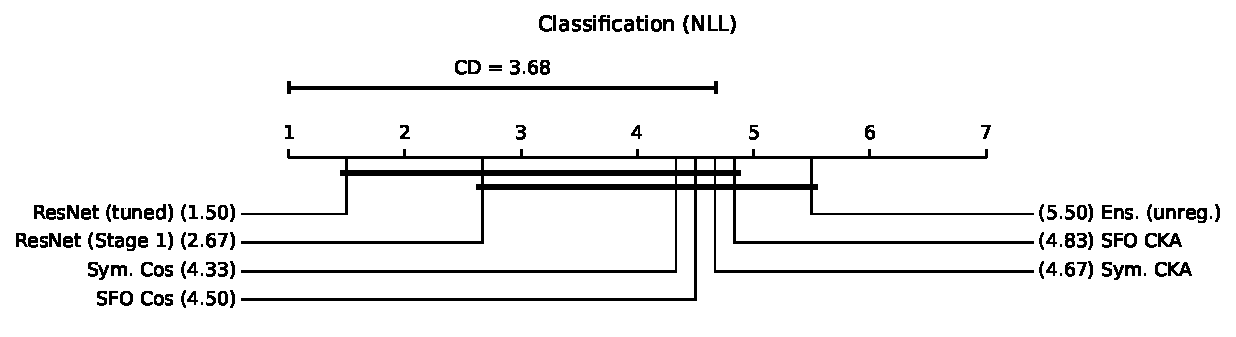
\includegraphics[width=0.75\textwidth]{figures/cd_classification.pdf}\\[1ex]
    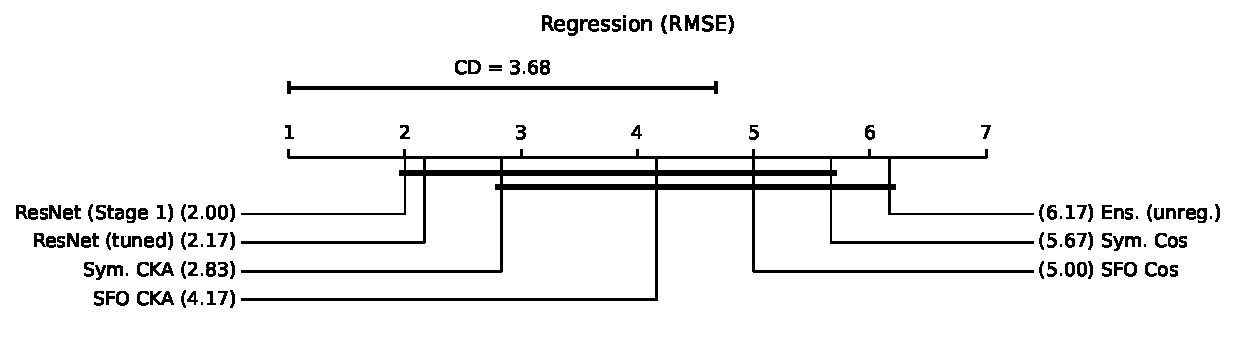
\includegraphics[width=0.75\textwidth]{figures/cd_regression.pdf}
    \caption{Critical difference diagrams (Nemenyi, $\alpha = 0.05$, $\text{CD} = 3.68$) of the mean ranks on classification NLL (top) and regression RMSE (bottom). Methods connected by a bar are not significantly different.}
    \label{fig:cd_tasks}
\end{figure}

\clearpage
\subsection{Ensemble Diagnostics}
Figure~\ref{fig:member_norms} shows the output norms of the members and Figure~\ref{fig:similarity} the pairwise similarity of their representations.

\begin{figure}[htbp]
    \centering
    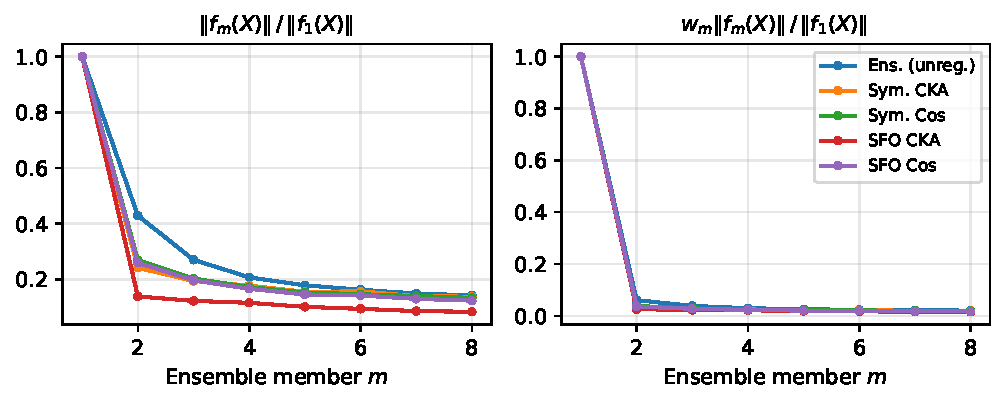
\includegraphics[width=0.9\textwidth]{figures/member_norms.pdf}
    \caption{Root-mean-square output norm of each member on the outer test fold relative to the first member, without (left) and with (right) the member weight $w_1 = 1$, $w_m = \nu$ for $m \ge 2$. Geometric mean over all $300$ runs per method.}
    \label{fig:member_norms}
\end{figure}

\begin{figure}[htbp]
    \centering
    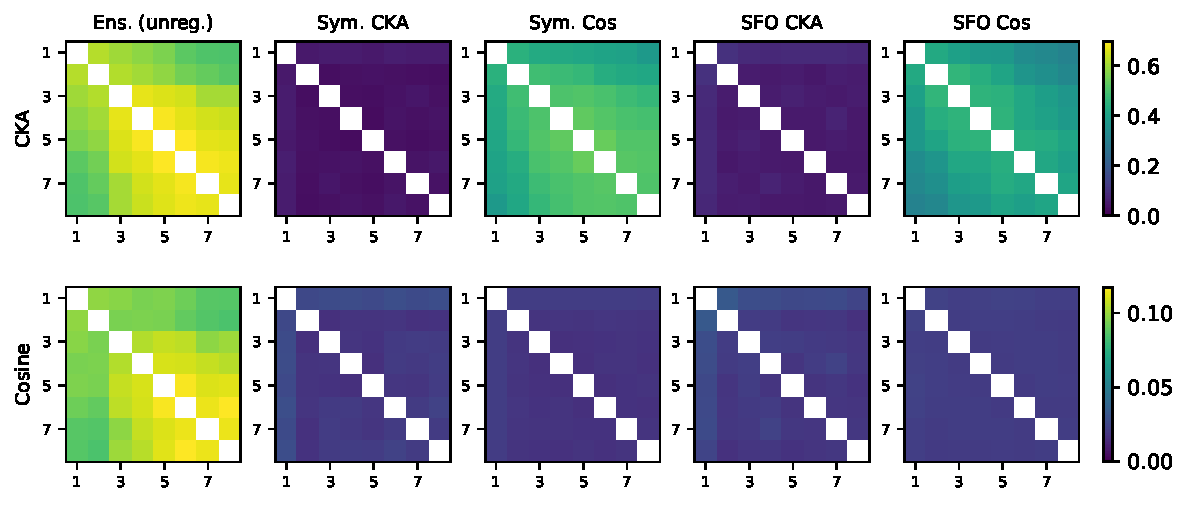
\includegraphics[width=\textwidth]{figures/similarity.pdf}
    \caption{Pairwise linear CKA (top) and squared cosine similarity (bottom) between the centered penultimate representations of the members on the outer test fold, averaged over all $300$ runs per method. The diagonal (equal to $1$) is omitted; each row shares one color scale.}
    \label{fig:similarity}
\end{figure}

\clearpage
\subsection{Stability, Cost and Selected Hyperparameters}
\label{app:other}
Table~\ref{tab:stability} compares the standard deviations of the primary metrics relative to ResNet (Stage 1): $\sigma$ over all fold--seed results, $\sigma_{\text{fold}}$ between the fold means and $\bar{\sigma}_{\text{seed}}$ between the seeds within a fold. Table~\ref{tab:cost} lists the number of trainable parameters, refit epochs and refit training time. Table~\ref{tab:hyperparameters_selected} and Figure~\ref{fig:hyperparameters} summarize the selected hyperparameters over the $60$ dataset--fold pairs.

\begin{table}[htbp]
    \centering
    \caption{Stability: geometric mean over datasets of the standard deviation of the primary metric (NLL / RMSE) relative to ResNet (Stage 1) (values below 1 are more stable). $\sigma$: over all $25$ fold--seed results; $\sigma_{\text{fold}}$: over the $5$ fold means; $\bar{\sigma}_{\text{seed}}$: mean over folds of the standard deviation over the $5$ seeds.}
    \label{tab:stability}
    \resizebox{\ifdim\width>\textwidth\textwidth\else\width\fi}{!}{%
    \begin{tabular}{lcccccc}
        \toprule
        \textbf{Method} & \multicolumn{3}{c}{\textbf{Classification (NLL)}} & \multicolumn{3}{c}{\textbf{Regression (RMSE)}} \\ \cmidrule(lr){2-4} \cmidrule(lr){5-7} & $\sigma$ & $\sigma_{\text{fold}}$ & $\bar{\sigma}_{\text{seed}}$ & $\sigma$ & $\sigma_{\text{fold}}$ & $\bar{\sigma}_{\text{seed}}$ \\
        \midrule
        ResNet (Stage 1) & 1.000 & 1.000 & 1.000 & \textbf{1.000} & 1.000 & \textbf{1.000} \\
        ResNet (tuned) & 0.993 & 1.138 & \textbf{0.848} & 1.014 & 0.977 & 1.005 \\
        Ens. (unreg.) & 1.166 & 1.217 & 1.412 & 1.433 & 1.407 & 1.497 \\
        Sym. CKA & 1.318 & 1.479 & 1.320 & 1.026 & \textbf{0.877} & 1.257 \\
        Sym. Cos & 1.750 & 1.779 & 1.817 & 1.303 & 1.285 & 1.417 \\
        SFO CKA & 1.322 & 1.514 & 1.118 & 1.181 & 0.961 & 1.388 \\
        SFO Cos & \textbf{0.912} & \textbf{0.964} & 1.020 & 1.368 & 1.174 & 1.668 \\
        \bottomrule
    \end{tabular}%
    }
\end{table}

\begin{table}[htbp]
    \centering
    \caption{Computational cost of the final refits: median over all $300$ refits per method, and geometric mean over datasets of the per-dataset mean relative to ResNet (Stage 1) ($\times$ref). Training time is the wall-clock time of the refit on a GPU.}
    \label{tab:cost}
    \resizebox{\ifdim\width>\textwidth\textwidth\else\width\fi}{!}{%
    \begin{tabular}{lcccccc}
        \toprule
        \textbf{Method} & \multicolumn{2}{c}{\textbf{Trainable parameters}} & \multicolumn{2}{c}{\textbf{Refit epochs}} & \multicolumn{2}{c}{\textbf{Training time [s]}} \\ \cmidrule(lr){2-3} \cmidrule(lr){4-5} \cmidrule(lr){6-7} & median & $\times$ref & median & $\times$ref & median & $\times$ref \\
        \midrule
        ResNet (Stage 1) & 136,578 & 1.00 & 72.0 & 1.00 & 2.4 & 1.00 \\
        ResNet (tuned) & 136,578 & 1.00 & 70.5 & 0.98 & 2.4 & 0.86 \\
        Ens. (unreg.) & 1,092,624 & 8.00 & 52.0 & 0.77 & 8.7 & 3.79 \\
        Sym. CKA & 1,092,624 & 8.00 & 68.0 & 0.94 & 15.1 & 5.17 \\
        Sym. Cos & 1,092,624 & 8.00 & 58.5 & 0.81 & 11.8 & 4.30 \\
        SFO CKA & 1,092,624 & 8.00 & 64.0 & 0.84 & 11.7 & 4.43 \\
        SFO Cos & 1,092,624 & 8.00 & 54.0 & 0.77 & 10.4 & 4.05 \\
        \bottomrule
    \end{tabular}%
    }
\end{table}

\begin{table}[htbp]
    \centering
    \small
    \setlength{\tabcolsep}{4pt}
    \caption{Selected hyperparameters: median and [first, third] quartile over the $60$ dataset--fold pairs. $\eta$: learning rate, $\gamma$: weight decay, $\nu$: additive coefficient, $\lambda$: penalty weight, $e^\star$: best inner-validation epoch (the refit length). The Stage~1 ResNet uses the fixed $\eta = 10^{-3}$, $\gamma = 10^{-4}$.}
    \label{tab:hyperparameters_selected}
    \resizebox{\ifdim\width>\textwidth\textwidth\else\width\fi}{!}{%
    \begin{tabular}{lccccc}
        \toprule
        \textbf{Method} & $\eta$ & $\gamma$ & $\nu$ & $\lambda$ & $e^\star$ \\
        \midrule
        ResNet (Stage 1) & -- & -- & -- & -- & \begin{tabular}[t]{@{}c@{}}72\\{\scriptsize [54, 97]}\end{tabular} \\
        ResNet (tuned) & \begin{tabular}[t]{@{}c@{}}$1.2{\times}10^{-3}$\\{\scriptsize [$4.7{\times}10^{-4}$, $1.9{\times}10^{-3}$]}\end{tabular} & \begin{tabular}[t]{@{}c@{}}$5.3{\times}10^{-5}$\\{\scriptsize [$9.8{\times}10^{-6}$, $1.1{\times}10^{-3}$]}\end{tabular} & -- & -- & \begin{tabular}[t]{@{}c@{}}70\\{\scriptsize [42, 106]}\end{tabular} \\
        Ens. (unreg.) & \begin{tabular}[t]{@{}c@{}}$1.2{\times}10^{-3}$\\{\scriptsize [$7.0{\times}10^{-4}$, $2.8{\times}10^{-3}$]}\end{tabular} & \begin{tabular}[t]{@{}c@{}}$6.7{\times}10^{-5}$\\{\scriptsize [$5.4{\times}10^{-6}$, $4.1{\times}10^{-4}$]}\end{tabular} & \begin{tabular}[t]{@{}c@{}}0.120\\{\scriptsize [0.064, 0.248]}\end{tabular} & -- & \begin{tabular}[t]{@{}c@{}}52\\{\scriptsize [32, 84]}\end{tabular} \\
        Sym. CKA & \begin{tabular}[t]{@{}c@{}}$1.2{\times}10^{-3}$\\{\scriptsize [$6.9{\times}10^{-4}$, $2.4{\times}10^{-3}$]}\end{tabular} & \begin{tabular}[t]{@{}c@{}}$2.4{\times}10^{-4}$\\{\scriptsize [$1.8{\times}10^{-5}$, $1.4{\times}10^{-3}$]}\end{tabular} & \begin{tabular}[t]{@{}c@{}}0.111\\{\scriptsize [0.076, 0.227]}\end{tabular} & \begin{tabular}[t]{@{}c@{}}$6.9{\times}10^{-2}$\\{\scriptsize [$9.2{\times}10^{-3}$, $5.9{\times}10^{-1}$]}\end{tabular} & \begin{tabular}[t]{@{}c@{}}68\\{\scriptsize [39, 86]}\end{tabular} \\
        Sym. Cos & \begin{tabular}[t]{@{}c@{}}$1.7{\times}10^{-3}$\\{\scriptsize [$7.2{\times}10^{-4}$, $3.1{\times}10^{-3}$]}\end{tabular} & \begin{tabular}[t]{@{}c@{}}$2.0{\times}10^{-4}$\\{\scriptsize [$1.4{\times}10^{-5}$, $1.3{\times}10^{-3}$]}\end{tabular} & \begin{tabular}[t]{@{}c@{}}0.125\\{\scriptsize [0.068, 0.252]}\end{tabular} & \begin{tabular}[t]{@{}c@{}}$2.0{\times}10^{-1}$\\{\scriptsize [$5.0{\times}10^{-3}$, $2.9{\times}10^{0}$]}\end{tabular} & \begin{tabular}[t]{@{}c@{}}58\\{\scriptsize [36, 90]}\end{tabular} \\
        SFO CKA & \begin{tabular}[t]{@{}c@{}}$9.9{\times}10^{-4}$\\{\scriptsize [$5.3{\times}10^{-4}$, $2.0{\times}10^{-3}$]}\end{tabular} & \begin{tabular}[t]{@{}c@{}}$1.2{\times}10^{-4}$\\{\scriptsize [$1.1{\times}10^{-5}$, $7.1{\times}10^{-4}$]}\end{tabular} & \begin{tabular}[t]{@{}c@{}}0.167\\{\scriptsize [0.084, 0.338]}\end{tabular} & \begin{tabular}[t]{@{}c@{}}$2.9{\times}10^{-1}$\\{\scriptsize [$1.2{\times}10^{-2}$, $2.1{\times}10^{0}$]}\end{tabular} & \begin{tabular}[t]{@{}c@{}}64\\{\scriptsize [35, 88]}\end{tabular} \\
        SFO Cos & \begin{tabular}[t]{@{}c@{}}$1.4{\times}10^{-3}$\\{\scriptsize [$8.3{\times}10^{-4}$, $2.7{\times}10^{-3}$]}\end{tabular} & \begin{tabular}[t]{@{}c@{}}$2.2{\times}10^{-4}$\\{\scriptsize [$8.7{\times}10^{-6}$, $2.7{\times}10^{-3}$]}\end{tabular} & \begin{tabular}[t]{@{}c@{}}0.125\\{\scriptsize [0.072, 0.215]}\end{tabular} & \begin{tabular}[t]{@{}c@{}}$1.8{\times}10^{-1}$\\{\scriptsize [$5.7{\times}10^{-3}$, $4.8{\times}10^{0}$]}\end{tabular} & \begin{tabular}[t]{@{}c@{}}54\\{\scriptsize [35, 81]}\end{tabular} \\
        \bottomrule
    \end{tabular}%
    }
\end{table}


\begin{figure}[htbp]
    \centering
    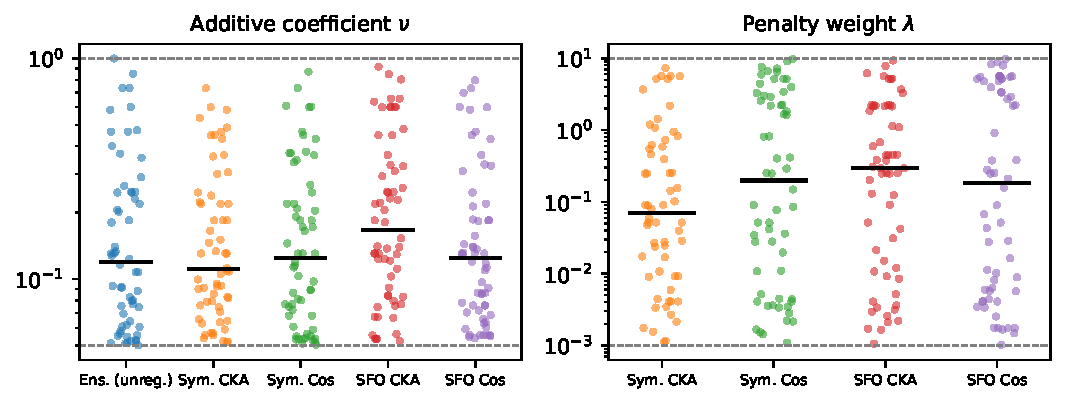
\includegraphics[width=0.85\textwidth]{figures/hyperparameters.pdf}
    \caption{Selected additive coefficient $\nu$ and penalty weight $\lambda$ for each of the $60$ dataset--fold pairs (points) and their median (black line). Dashed lines mark the bounds of the search range.}
    \label{fig:hyperparameters}
\end{figure}

\end{document}


